% Convergent null results for single-cluster industrial nowcasting from satellite NO2.
% Self-contained working paper. Compile with tectonic (runs the full pipeline automatically):
%     tectonic nox_convergent_nulls.tex
% or with a TeX Live toolchain:
%     pdflatex nox_convergent_nulls  (run twice)
% Figures are drawn natively with pgfplots, except figures/wide_ring_sensitivity.png,
% which ships alongside this file so the source directory is self-contained.
\documentclass[11pt,a4paper]{article}

\usepackage[utf8]{inputenc}
\usepackage[T1]{fontenc}
\usepackage{lmodern}
\usepackage[margin=2.4cm]{geometry}
\usepackage{graphicx}
\usepackage{booktabs}
\usepackage{amsmath}
\usepackage{caption}
\usepackage{subcaption}
\usepackage{xcolor}
\usepackage{pgfplots}
\pgfplotsset{compat=1.17}
\usepackage[round,authoryear]{natbib}
\usepackage[hidelinks]{hyperref}
\usepackage{authblk}
\usepackage{enumitem}

\captionsetup{font=small,labelfont=bf}
\setlength{\parskip}{0.35em}
% Absorb the few long unbreakable tokens (identifiers, URLs) without ragged-right.
\setlength{\emergencystretch}{1.2em}

% Lightweight notation helpers. Units are set as plain text with a thin space; no siunitx
% dependency and no macro that has to be defeated for ranges such as 117.96--119.05 degE.
\providecommand{\degree}{\ensuremath{^{\circ}}}
\newcommand{\rval}[1]{\mbox{$r=#1$}}
\providecommand{\doi}[1]{DOI:~\href{https://doi.org/#1}{#1}}
\providecommand{\ce}[1]{\ensuremath{\mathrm{#1}}}

% Single point of truth for the reproducibility anchor. Update after committing the
% derived artefacts enumerated in the Data and code availability section.
\newcommand{\repocommit}{\texttt{b4c1dd7}}

\definecolor{noxink}{HTML}{0F6B73}
\definecolor{noxember}{HTML}{A8492C}
\definecolor{noxgrey}{HTML}{6B6B6B}

\title{\bfseries Non-separability of a single industrial cluster from its regional
background in satellite \ce{NO_2}: a null result over Tangshan, China}

\author[1]{A.~Betato}
\affil[1]{Independent researcher --- \texttt{abetatos@gmail.com}}
\date{31 August 2026}

\begin{document}
\maketitle

\begin{abstract}
\noindent
Tropospheric \ce{NO_2} from Sentinel-5P/TROPOMI is an established proxy for combustion activity
and is increasingly proposed as a real-time economic nowcast. We test a deliberately harder,
single-cluster case: whether a strictly public, free-data analysis can isolate the activity signal
of \emph{one} industrial cluster --- the Tangshan blast-furnace (BF) complex in Hebei, China (39
located facilities, 26 active) --- and validate it against an independent physical benchmark, the
BF operating rate published by the Centre for Research on Energy and Clean Air (CREA). Five
analyses, each targeting a different route by which the signal might be recovered, were computed
blind to the benchmark at parameters fixed beforehand and judged under autocorrelation-robust
inference. All five are negative. We report the outcome as an \emph{exclusion} rather than a
failure to reject: at an effective sample size of $\approx289$ weeks, these data rule out any
weekly linear coupling above \rval{0.17} (upper 95\% bootstrap bound), i.e.\ under 3\% of shared
variance. A change-variance decomposition attributes 93--95\% of the footprint's week-to-week
variance to a regional common mode. A hard-to-falsify thermal proxy (public NASA active-fire data)
tracks neither \ce{NO_2} nor the benchmark, because it observes agricultural crop-residue burning
rather than furnaces. The encouraging 2023 peak in a rolling correlation reaches only \rval{0.276}
and is unremarkable under a rolling-window scan-maximum null ($p=0.325$). A forecasting-skill
screen finds no \ce{NO_2} feature that adds information over the operational benchmark. Finally
\ce{NO_2} flux divergence \citep{beirle_2021,beirle_2023} returns a non-detection at the four real
overpasses we could obtain. The near-null is not an artefact of the target: the CREA Tangshan rate
tracks a separately surveyed 247-mill national panel at \rval{0.76} in weekly changes, so
measurement error in the benchmark cannot account for a feature correlation of $0.08$. We are
explicit that the five results are \emph{not} statistically independent --- they share one
\ce{NO_2} cube, one background ring and one benchmark --- so their convergence is corroboration
only against the failure modes they do \emph{not} share (Section~\ref{sec:shared}), and we
enumerate those. Two discriminating controls run against our own interpretation did not
corroborate the spatial explanation: sweeping the background-ring radii to 150\,km on a
$4.8\times$ larger cube shows the cluster-local variance share is \emph{ring-dependent} and still
rising at the edge of the domain, and scoring the same features against national steel activity
shows they track the national target no better than Tangshan's own. We therefore report spatial
non-separability at TROPOMI's resolution as the leading hypothesis rather than an established
cause, and state precisely what would settle it --- a geostationary, higher-contrast \ce{NO_2}
sensor \citep{kim_2020_gems,park_2025_gems_gan}.

\vspace{4pt}\noindent\textbf{Keywords:} tropospheric \ce{NO_2}; TROPOMI; economic nowcasting;
iron and steel; null results; equivalence bounds; source attribution; flux divergence.
\end{abstract}

\section{Introduction}
\label{sec:intro}

\paragraph{Premise.} Satellite \ce{NO_2} is a combustion tracer, and a small literature uses it as
an economic nowcast: at national scale for China
\citep{morris_zhang_2019,li_zheng_2023,li_2024_nox_trends}, across global cities
\citep{montgomery_holloway_2018}, and as an industrial-shock read for Ukraine
\citep{mao_2025_ukraine}; the broad case for satellite data in economics is made by
\citet{donaldson_storeygard_2016} and \citet{ezran_2023}. We ask a harder, single-cluster
question: can the \ce{NO_2} column over one industrial cluster --- the Tangshan blast-furnace
complex, the largest steel agglomeration in China ($\sim$13\% of national output) --- track that
cluster's physical output at a useful frequency, using only public, free data?

\paragraph{Why it is hard.} Tangshan sits inside the Beijing--Tianjin--Hebei (BTH) plume, one of
the most \ce{NO_2}-loaded airsheds on Earth. Steel is only $\sim$30--43\% of the cluster's own
\ce{NO_2} column \citep{wen_2024}; traffic, power and residential sources fill the rest, and an
ultra-low-emission retrofit programme is reported to drive a secular intensity decline that
decouples emissions from output \citep{li_2024_nox_trends}. A validation is also only as good as
its target, and the natural benchmark --- the CREA BF operating rate
\citep{crea_steel_benchmark} --- is a commercial trader survey, so any near-null could be blamed
on either the feature or the target. We therefore adopt a fixed analysis protocol
(Section~\ref{sec:methods}) and treat a well-characterised null as a valid, reportable outcome
\citep{morris_zhang_2019}.

\paragraph{Contribution and its limits.} This paper reports five analyses, each targeting a
different recovery route, and shows that they converge on one physical explanation.
Table~\ref{tab:glance} is the map. We are deliberately careful about what that convergence buys:
the five share their inputs, so they are not five independent draws on the same hypothesis.
Section~\ref{sec:shared} sets out which failure modes are shared and which are not, and
Section~\ref{sec:limitations} lists, without hedging, the controls that would discriminate the
remaining alternatives and that this study did not run.

\begin{table}[t]
\centering
\caption{Overview of the five analyses. Each targets a different recovery route; all are computed
blind to the validation benchmark and judged under autocorrelation-robust inference
(Section~\ref{sec:methods}). Three cross-cutting checks support all five rather than adding a sixth
analysis: a spatial-scale sweep (Section~\ref{sec:scale}), a background-ring radius sweep
(Section~\ref{sec:ringsweep}) and a wider-scale benchmark contrast
(Section~\ref{sec:scalecontrast}). The five are not statistically independent: see
Section~\ref{sec:shared}.}
\label{tab:glance}
\small
\begin{tabular}{p{0.16\linewidth}p{0.26\linewidth}p{0.30\linewidth}p{0.16\linewidth}}
\toprule
Analysis & What it tests & Key statistic & Finding \\
\midrule
Variance attribution & Cluster share of change-variance &
regional 0.93--0.95; cluster-local $\le0.014$ (95\% bd.) at 25--60\,km, $0.061$ at 90--150\,km &
regional mode dominates; share is ring-dependent \\
\addlinespace
Thermal proxy & Independent thermal signature of furnaces &
\ce{NO_2}$\leftrightarrow$fire \rval{-0.054}; CREA$\leftrightarrow$fire \rval{-0.049} (ns) &
proxy uninformative \\
\addlinespace
Regime stability & Robustness of the 2023 correlation peak &
peak \rval{0.276}; scan-max $p=0.325$ & unremarkable under scan-max null \\
\addlinespace
Forecasting skill & Lead/skill over the operational benchmark &
\rval{-0.014}\,/\,$+0.063$; $|r|>0.17$ excluded & no incremental info \\
\addlinespace
Flux inversion & A separable point source above background &
noise $\downarrow3.4\times$; SNR $\approx+0.27$ at $N{=}4$ & no source detected at $N{=}4$ \\
\bottomrule
\end{tabular}
\end{table}

\section{Data and study region}
\label{sec:data}

\paragraph{Study region.} The area of interest (AOI) encloses the 39 located Tangshan
blast-furnace facilities (117.96--119.05\,\degree E, 38.95--40.21\,\degree N) plus a
0.25\,\degree{} buffer, on the North China Plain in Hebei (Fig.~\ref{fig:map}). Of the 39, 26
are active (25 \emph{operating} plus one \emph{operating pre-retirement}) and define the
analysis footprint: the union of 15\,km discs around the active facilities (448 of the
1{,}530 AOI grid cells). A concentric
25--60\,km background ring around that footprint provides the regional-background reference used
throughout. Analysis uses TROPOMI's native retrieval grid ($\sim$4--6\,km). The choice of ring
radii is the single most consequential free geometric parameter in this study; it is examined
critically in Section~\ref{sec:ringcaveat} and swept in Section~\ref{sec:ringsweep}, which required
re-acquiring the record over a $1.25\degree$ buffer because the AOI defined here is too small to
form a complete annulus beyond 63\,km.

\begin{figure}[t]
\centering
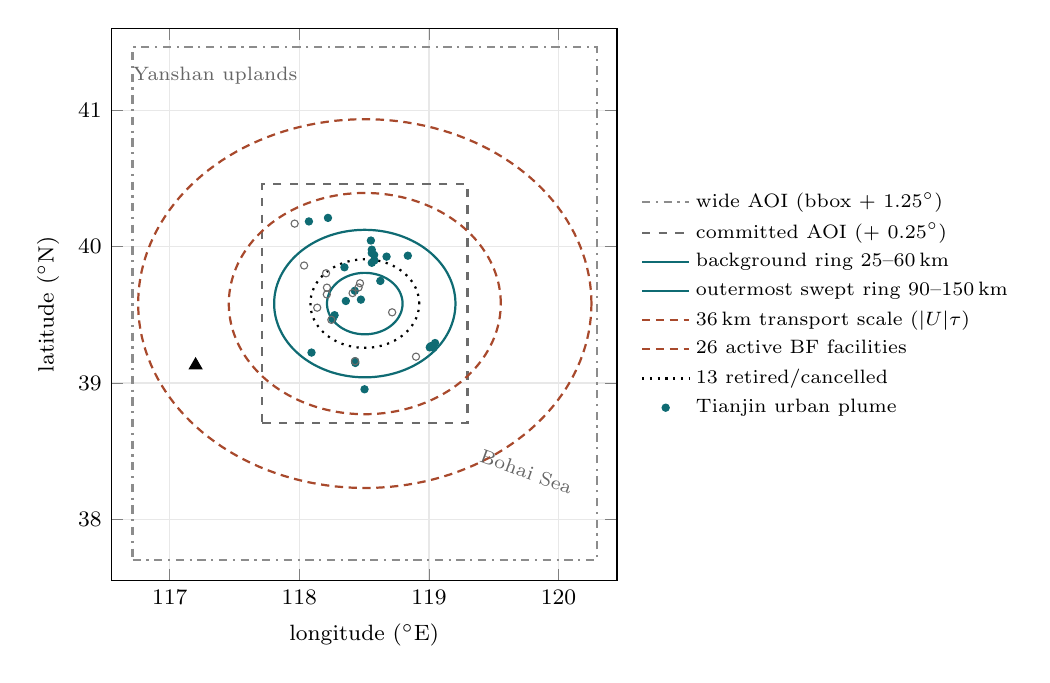
\begin{tikzpicture}
\begin{axis}[
  width=0.66\linewidth, height=8.6cm,
  xlabel={longitude (\degree E)}, ylabel={latitude (\degree N)},
  xmin=116.55, xmax=120.45, ymin=37.55, ymax=41.60,
  axis equal image=false,
  tick label style={font=\footnotesize}, label style={font=\footnotesize},
  legend style={at={(1.03,0.5)},anchor=west,draw=none,font=\scriptsize,cells={anchor=west}},
  ymajorgrids, xmajorgrids, grid style={gray!18},
]
% Wide AOI re-acquired for the ring sweep: facility bbox + 1.25 deg.
\addplot[black!45, thick, dash dot] coordinates
  {(116.714,37.704) (120.297,37.704) (120.297,41.460) (116.714,41.460) (116.714,37.704)};
\addlegendentry{wide AOI (bbox $+$ 1.25\degree)}
% Committed AOI: facility bbox + 0.25 deg.
\addplot[noxgrey, thick, dashed] coordinates
  {(117.714,38.704) (119.297,38.704) (119.297,40.460) (117.714,40.460) (117.714,38.704)};
\addlegendentry{committed AOI ($+$ 0.25\degree)}
% Committed background ring, 25--60 km.
\addplot[noxink, thick, domain=0:360, samples=160] ({118.505+0.2914*cos(x)}, {39.582+0.2252*sin(x)});
\addplot[noxink, thick, domain=0:360, samples=160] ({118.505+0.6993*cos(x)}, {39.582+0.5405*sin(x)});
\addlegendentry{background ring 25--60\,km}
% Outermost swept ring, 90--150 km.
\addplot[noxember, thick, densely dashed, domain=0:360, samples=160] ({118.505+1.0490*cos(x)}, {39.582+0.8108*sin(x)});
\addplot[noxember, thick, densely dashed, domain=0:360, samples=160] ({118.505+1.7483*cos(x)}, {39.582+1.3514*sin(x)});
\addlegendentry{outermost swept ring 90--150\,km}
% Mean advection scale |U|tau ~ 36 km: it falls INSIDE the committed ring.
\addplot[black, thick, dotted, domain=0:360, samples=160] ({118.505+0.4196*cos(x)}, {39.582+0.3243*sin(x)});
\addlegendentry{36\,km transport scale ($|U|\tau$)}
\addplot[only marks, mark=*, mark size=1.3pt, noxink] coordinates {
(118.503,38.954) (118.432,39.147) (118.430,39.160) (118.094,39.223) (119.034,39.258) (119.006,39.261)
(119.025,39.268) (119.014,39.270) (119.047,39.293) (118.257,39.468) (118.272,39.497) (118.359,39.601)
(118.475,39.611) (118.428,39.676) (118.625,39.748) (118.348,39.848) (118.559,39.881) (118.579,39.898)
(118.673,39.926) (118.837,39.933) (118.577,39.939) (118.559,39.952) (118.559,39.977) (118.552,40.044)
(118.074,40.184) (118.221,40.210)
};
\addlegendentry{26 active BF facilities}
\addplot[only marks, mark=o, mark size=1.3pt, noxgrey] coordinates {
(118.430,39.160) (118.900,39.193) (118.247,39.463) (118.716,39.518) (118.138,39.552) (118.212,39.649)
(118.411,39.659) (118.213,39.699) (118.457,39.700) (118.468,39.731) (118.206,39.804) (118.037,39.861)
(117.964,40.168)
};
\addlegendentry{13 retired/cancelled}
% Confounders the outermost ring reaches.
\addplot[only marks, mark=triangle*, mark size=2.6pt, black] coordinates {(117.20,39.13)};
\addlegendentry{Tianjin urban plume}
\node[font=\scriptsize, black!60, anchor=center, rotate=-20] at (axis cs:119.75,38.35) {Bohai Sea};
\node[font=\scriptsize, black!60, anchor=center] at (axis cs:117.35,41.25) {Yanshan uplands};
\end{axis}
\end{tikzpicture}
\caption{Study geometry, and the geometric confound the ring sweep runs into. The analysis
footprint is the union of 15\,km discs around the 26 active blast-furnace facilities (filled
markers); the background reference of record is the 25--60\,km ring (teal). The dotted circle is
the mean advection scale implied by the flux analysis (mean effective wind $|U|=2.48$\,m\,s$^{-1}$
times the assumed \ce{NO_2} lifetime $\tau=4$\,h, i.e.\ $\approx36$\,km): it falls \emph{inside}
the background ring, which is the self-subtraction concern of Section~\ref{sec:ringcaveat}(i).
The outermost ring the sweep could form (ember, 90--150\,km; Section~\ref{sec:ringsweep}) escapes
the advection scale but no longer samples the same air mass --- it spans the Bohai Sea to the
south-east and reaches the Tianjin urban plume to the west. That trade-off, not computation, is
why the sweep stops at 150\,km. Rings are drawn in ground distance about the cluster centroid.}
\label{fig:map}
\end{figure}

\paragraph{\ce{NO_2} data and processor versions.} Tropospheric \ce{NO_2} was acquired from the
Copernicus Data Space Ecosystem (CDSE) \texttt{SENTINEL\_5P\_L2} collection through openEO,
server-side clipped to the AOI, and screened at \texttt{qa\_value} $\ge0.75$. The archive
comprises 2{,}641 AOI-intersecting overpasses from 2019-01-01 to 2026-06-12, composited without
interpolation to a weekly cube (389 weeks) and a daily cube. Individual Level-2 orbit swaths,
obtained separately from the CDSE OData/zipper route, supply per-overpass fields for the flux
analysis.

We state plainly a limitation a reviewer will otherwise find: \textbf{the record is not
processor-version homogenised.} The openEO collection does not expose a per-overpass processor
version, so our manifest labels overpasses by a fixed 2022-07-01 cutoff
(1{,}219 labelled \texttt{v1.x}, 1{,}422 \texttt{v2.x}). The record therefore spans the
v1.2, v1.3, v1.4 and v2.x processor sequence, and no correction for the known
step change in tropospheric columns at the v2 transition (and the associated PAL reprocessing)
was applied. Every result reported here is a \emph{correlation or variance share} between two
series measured on the same cube, which a common multiplicative level shift largely divides out;
but any statement about a secular \emph{trend} in the \ce{NO_2} level is confounded with this
version sequence, and we withdraw such statements accordingly (Section~\ref{sec:baseline}).

\paragraph{Other data.} (i) \emph{Benchmark}: the CREA Tangshan BF operating rate
\citep{crea_steel_benchmark}, weekly, the only Tangshan-specific public physical-output series;
CREA also publishes national aggregates (Section~\ref{sec:limitations}). (ii)
\emph{Meteorology}: ERA5 single-levels 10\,m winds and boundary-layer height
\citep{hersbach_2020_era5,cds_era5}, used as the ventilation covariate and, for the flux product,
the advecting wind. (iii) \emph{Thermal}: NASA active-fire detections (90{,}895 over 2019--2026)
as a candidate physical proxy.

\paragraph{Sample sizes.} Different analyses use different subsets, and the counts do not
coincide. Table~\ref{tab:n} reconciles every $n$ quoted in this paper to its cause, so that no
sample size appears without an accounted-for provenance.

\begin{table}[t]
\centering
\caption{Reconciliation of every sample size in this paper. Each row is the count after applying
the stated screen to the row above it within its block. No observation is imputed or
interpolated anywhere in the pipeline.}
\label{tab:n}
\small
\begin{tabular}{@{}l p{0.68\linewidth} r@{}}
\toprule
Block & Screen applied & $n$ \\
\midrule
\multicolumn{3}{l}{\emph{Daily cube (Section~\ref{sec:variance})}}\\
& calendar days spanned, 2019-01-01 to 2026-06-12 & 2{,}720 \\
& days with a valid footprint \emph{and} ring value after cloud/QA screening & 2{,}007 \\
& \quad$\hookrightarrow$ minus days lacking ERA5 covariates \; (deseason $\cdot$ daily) & 2{,}003 \\
& of the 2{,}007, those with a valid \emph{immediately preceding} day & 1{,}559 \\
& \quad$\hookrightarrow$ minus days lacking ERA5 covariates \; (first-diff $\cdot$ daily) & 1{,}555 \\
\addlinespace
\multicolumn{3}{l}{\emph{Weekly cube}}\\
& weekly composite periods, 2019-01 to 2026-06 & 389 \\
& \quad$\hookrightarrow$ minus one period lost to differencing (first-diff $\cdot$ weekly) & 388 \\
& \quad$\hookrightarrow$ weeks jointly observed with the CREA benchmark & 379 \\
& \quad\quad$\hookrightarrow$ minus weeks below the 0.25 valid-coverage screen & 364 \\
& \quad$\hookrightarrow$ weeks jointly observed with the active-fire series (ends 2026-05-03) & 373 \\
\bottomrule
\end{tabular}
\end{table}

\noindent The weekly cells of Table~\ref{tab:variance} use 389 (deseason) and 388 (first
difference) because the variance decomposition never touches the benchmark and so is not subject
to the CREA-overlap or coverage screens. Table~\ref{tab:nowcast} uses 364 for the
background-corrected residual (which carries a \texttt{valid\_coverage} column and is screened)
and 379 for the intensity-decomposition covariate (which does not), and this is the whole of the
difference between those two rows.

\section{Methods}
\label{sec:methods}

\paragraph{Estimation blind to the benchmark.} Every feature, decomposition and screening
statistic is computed from \ce{NO_2}, meteorology and background alone; the CREA series is used
only at the final scoring step. No parameter anywhere in the feature path is tuned to the
benchmark. This guards against selecting a signal into existence.

\paragraph{The three \ce{NO_2} features, and how they differ.} Three derived series appear in this
paper, and because two of them are scored at the same $n$ against the same benchmark we define all
three here rather than let the reader infer them from context.

\begin{enumerate}[leftmargin=1.6em,itemsep=0.2em,label=(\roman*)]
  \item \textbf{Background-corrected residual} (\texttt{no2\_corrected}): the footprint column
  minus the concentric background-ring column, period by period. This is the raw spatial contrast,
  with no temporal model applied.
  \item \textbf{\ce{NO_2} activity index} (\texttt{index\_value}): the background-corrected
  residual after removing an annual harmonic, a heating-season structural term and a linear
  meteorological control (10\,m winds, wind speed, boundary-layer height). This is the feature of
  record for the coupling tests.
  \item \textbf{Intensity-decomposition covariate} (\texttt{residual\_activity}): the activity
  component of the intensity decomposition. It is the \emph{same series} as the activity index up
  to a fixed scale factor --- their correlation is $0.999993$ --- and we say so plainly, because
  earlier drafts reported the two as though they were independent features.
\end{enumerate}

\noindent It follows that the two headline weekly correlations against the benchmark, $+0.078$ and
$+0.063$, are one feature under two screens, not two features: $+0.078$ ($n=364$) applies the
$0.25$ valid-coverage screen, $+0.063$ ($n=379$) does not. Only (i), at $-0.014$ ($n=364$), is a
genuinely different quantity. All three are reproduced by
\texttt{analysis/benchmark\_reliability.py} from the committed series.

\paragraph{Autocorrelation-robust inference.} Both series are strongly serially correlated (for
the weekly activity index against the benchmark, effective sample size $n_{\text{eff}}=288.7$
of $n=364$), so the naive Pearson $p$ overstates significance. All coupling tests report,
alongside the naive $r$: an effective sample size $n_{\text{eff}}=n(1-ab)/(1+ab)$ (with $a,b$ the
lag-1 autocorrelations) and a Newey--West heteroskedasticity- and autocorrelation-consistent
variant \citep{newey_west_1987}; a moving-block bootstrap 95\% confidence interval (CI) for $r$
\citep{kunsch_1989}; a block-permutation null $p$; and a Benjamini--Hochberg false-discovery-rate
(FDR) correction across the test family \citep{benjamini_hochberg_1995}. A single implementation of
this inference is applied unchanged across all five analyses --- which is convenient for
consistency and is also, as Section~\ref{sec:shared} notes, a shared failure mode.

\paragraph{Reporting nulls as exclusions, not as failures to reject.} A non-significant $p$ is not
a result; the quantity that is, is the largest effect the data can rule out. For every coupling
test we therefore report the upper bound of the moving-block bootstrap CI on $|r|$ and the share of
common variance it implies, alongside the minimum detectable correlation
$1.96/\sqrt{n_{\text{eff}}-3}$ that the design could have called significant. Across the three
features of the preceding paragraph the widest such bound is $0.167$ (activity index, screened;
CI $[-0.024,+0.167]$, $n_{\text{eff}}=288.7$, minimum detectable $|r|=0.116$). The citable form of
this paper's central null is therefore \emph{an observed weekly coupling of $+0.078$ with any
coupling above $|r|=0.17$ excluded at 95\% confidence --- under 2.8\% of shared variance} --- and
not ``no significant relationship was found''. Table~\ref{tab:equivalence} collects the bounds.

\paragraph{Fixed-parameter, benchmark-blind screens.} Each analysis begins with a low-cost screen
computed blind to the benchmark. Where a screen returns a null, the more elaborate model it would
otherwise have justified is not pursued, and we report the screen result. Every parameter ---
window lengths, thresholds, block sizes, random seeds, 5{,}000 bootstrap and permutation draws
--- is a compiled-in default fixed in the codebase before the benchmark was read, so the decision
to stop is determined by the data rather than by post-hoc choice.

\textbf{This is not preregistration.} There is no public registry entry, timestamp or protocol
DOI for this study. Fixed seeds and compiled-in defaults are a weaker guarantee than a registered
protocol: they establish that we did not tune parameters after seeing each outcome, but they
cannot establish the order in which analyses were conceived. We use ``fixed-parameter,
benchmark-blind'' throughout and avoid the word ``preregistered'', which we would not be able to
support.

\paragraph{Sequential variance partition.} The change-variance decomposition
(Section~\ref{sec:variance}) is a nested-OLS partition in a \emph{fixed order}:
regional\,$\to$\,meteorological\,$\to$\,cluster-local. Order matters. Variance shared between the
regional term and the cluster-local term is attributed entirely to whichever enters first, which
is the regional term by construction. The reported cluster-local share is therefore an estimate
of the \emph{incremental} explanatory power of a local term after the ring, not of the cluster's
total contribution, and it is a lower bound on the latter. Section~\ref{sec:ringcaveat} explains
why, for this geometry, that distinction is not cosmetic.

\section{Baseline coupling}
\label{sec:baseline}

Before the decompositions, the plain result (Fig.~\ref{fig:ts}). At the matched weekly cadence
the deseasonalised, meteorology-controlled \ce{NO_2} activity index tracks the BF rate at
\rval{0.078} ($n=364$, block-permutation $p=0.21$, bootstrap 95\% CI $[-0.024,+0.167]$);
monthly, \rval{0.157} ($n=90$, $p=0.24$, CI $[-0.079,+0.325]$). Neither is significant under any
of the robust criteria. Stated as an exclusion rather than a non-rejection
(Section~\ref{sec:methods}): these data rule out any weekly linear coupling above $|r|=0.17$,
i.e.\ more than $2.8\%$ of shared variance, at 95\% confidence
(Table~\ref{tab:equivalence}).

\begin{table}[t]
\centering
\caption{Equivalence bounds for every \ce{NO_2} feature scored against the CREA benchmark, weekly.
``excl.\ $|r|>$'' is the larger absolute end of the moving-block bootstrap 95\% CI --- the
smallest coupling the data are able to rule out --- and $r^2$ is the share of common variance it
corresponds to. ``MDC'' is the minimum detectable correlation $1.96/\sqrt{n_{\text{eff}}-3}$ at
the autocorrelation-adjusted effective sample size, i.e.\ the smallest $|r|$ this design could
have called significant. Features (i)--(iii) are defined in Section~\ref{sec:methods}; rows two
and four are the same series under two coverage screens. Reproduced by
\texttt{analysis/benchmark\_reliability.py}.}
\label{tab:equivalence}
\small
\begin{tabular}{@{}lrrrcrr@{}}
\toprule
Feature & $n$ & $n_{\text{eff}}$ & $r$ & boot 95\% CI & excl.\ $|r|>$ & MDC \\
\midrule
Background-corrected residual (i)          & 364 & 295.1 & $-0.0138$ & $[-0.120,+0.081]$ & 0.120 & 0.115 \\
\ce{NO_2} activity index (ii), screened    & 364 & 288.7 & $+0.0778$ & $[-0.024,+0.167]$ & 0.167 & 0.116 \\
\ce{NO_2} activity index (ii), unscreened  & 379 & 291.3 & $+0.0624$ & $[-0.049,+0.157]$ & 0.157 & 0.115 \\
Intensity-decomp.\ covariate (iii)         & 379 & 291.3 & $+0.0625$ & $[-0.049,+0.157]$ & 0.157 & 0.115 \\
\bottomrule
\end{tabular}
\end{table}

\paragraph{On the ``decoupling''.} The raw footprint \ce{NO_2} \emph{level} correlates negatively
with the BF rate over the whole record (monthly \rval{-0.276}, $n=90$), and an earlier partial
record put this at $-0.35$. Splitting the record removes most of the sign: 2019--2021
\rval{+0.168} ($n=36$), 2022--2026 \rval{-0.089} ($n=54$). Subtracting the background ring
removes it almost entirely (monthly \rval{-0.032}). A whole-sample negative that disappears both
within sub-periods and after background subtraction is what two slowly diverging series look
like, not a within-period inverse relationship.

We previously read that divergence as physical --- \ce{NO_2} falling with ultra-low-emission
retrofits while output rose. \textbf{We withdraw that reading here.} As
Section~\ref{sec:data} sets out, the 2019--2026 \ce{NO_2} record spans an unharmonised TROPOMI
processor-version sequence whose v2 transition is known to shift tropospheric columns by roughly
10--15\%, in the same direction and on the same timescale. A secular trend in the level cannot be
attributed to emissions rather than to retrieval versioning with these data. The correlation and
variance-share results below are unaffected --- they are computed from co-temporal contrasts
between the footprint and its own ring, both drawn from the same retrieval --- but the trend
narrative is not supportable and we do not rely on it.

\paragraph{The one encouraging structure.} A rolling correlation of the deseasonalised residual
against the BF rate is regime-dependent (Fig.~\ref{fig:ts}b). On the complete record, with the
78-week window and the deseasonalisation method of record, it ranges from $-0.124$ to $+0.276$,
peaking on 2023-08-27. An exploratory earlier pass on a partial record, monthly and differently
detrended, reported a swing from $-0.42$ to $+0.73$ and thus appeared to cross the 0.5--0.75
range reported in the nowcasting literature; on the complete record with fixed parameters it does
not come close. Section~\ref{sec:regime} tests whether even the $+0.276$ peak is more than
favourable-window noise.

\begin{figure}[t]
\centering
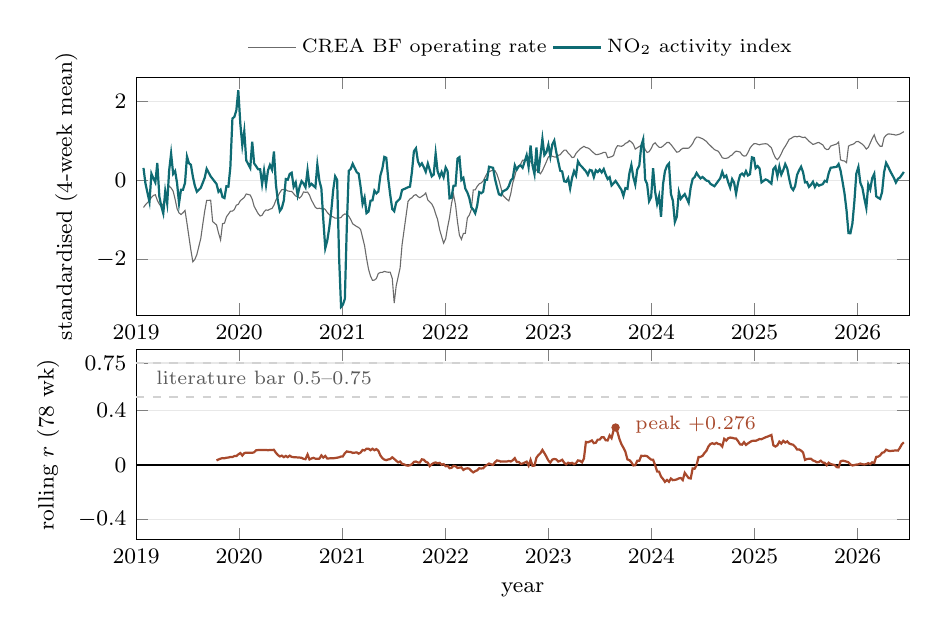
\begin{tikzpicture}
\begin{axis}[
  name=tsa,
  width=0.94\linewidth, height=4.6cm,
  xlabel={}, ylabel={standardised (4-week mean)},
  xmin=2019.0, xmax=2026.5, ymin=-3.4, ymax=2.6,
  xtick={2019,2020,2021,2022,2023,2024,2025,2026},
  scaled x ticks=false, x tick label style={/pgf/number format/1000 sep={}},
  tick label style={font=\footnotesize}, label style={font=\footnotesize},
  ymajorgrids, grid style={gray!18},
  legend style={at={(0.5,1.04)},anchor=south,draw=none,font=\scriptsize,legend columns=2},
]
\addplot[noxgrey, thin] coordinates {
(2019.071,-0.682) (2019.090,-0.614) (2019.129,-0.509) (2019.148,-0.426) (2019.167,-0.379)
(2019.186,-0.360) (2019.205,-0.499) (2019.225,-0.599) (2019.244,-0.659) (2019.263,-0.585)
(2019.282,-0.424) (2019.301,-0.277) (2019.320,-0.141) (2019.339,-0.188) (2019.359,-0.271)
(2019.378,-0.476) (2019.397,-0.712) (2019.416,-0.819) (2019.435,-0.859) (2019.454,-0.817)
(2019.474,-0.757) (2019.493,-1.080) (2019.512,-1.423) (2019.531,-1.760) (2019.550,-2.052)
(2019.569,-1.994) (2019.589,-1.869) (2019.627,-1.463) (2019.646,-1.110) (2019.665,-0.777)
(2019.684,-0.502) (2019.723,-0.500) (2019.742,-1.036) (2019.780,-1.123) (2019.799,-1.323)
(2019.819,-1.501) (2019.838,-1.091) (2019.857,-1.078) (2019.876,-0.918) (2019.895,-0.850)
(2019.914,-0.777) (2019.934,-0.773) (2019.953,-0.733) (2019.972,-0.623) (2019.991,-0.602)
(2020.011,-0.509) (2020.030,-0.470) (2020.049,-0.427) (2020.068,-0.340) (2020.107,-0.368)
(2020.126,-0.474) (2020.145,-0.654) (2020.183,-0.835) (2020.203,-0.897) (2020.222,-0.878)
(2020.241,-0.793) (2020.260,-0.744) (2020.279,-0.753) (2020.298,-0.724) (2020.318,-0.707)
(2020.337,-0.625) (2020.356,-0.493) (2020.375,-0.405) (2020.394,-0.305) (2020.413,-0.233)
(2020.433,-0.224) (2020.452,-0.234) (2020.471,-0.264) (2020.490,-0.274) (2020.509,-0.277)
(2020.528,-0.332) (2020.548,-0.395) (2020.567,-0.403) (2020.586,-0.445) (2020.605,-0.390)
(2020.624,-0.289) (2020.643,-0.300) (2020.663,-0.293) (2020.682,-0.370) (2020.701,-0.496)
(2020.720,-0.586) (2020.739,-0.680) (2020.758,-0.711) (2020.778,-0.700) (2020.797,-0.716)
(2020.816,-0.701) (2020.835,-0.732) (2020.854,-0.807) (2020.873,-0.860) (2020.893,-0.904)
(2020.912,-0.922) (2020.931,-0.952) (2020.950,-0.952) (2020.969,-0.948) (2020.988,-0.934)
(2021.005,-0.877) (2021.025,-0.844) (2021.044,-0.862) (2021.063,-0.901) (2021.082,-0.986)
(2021.101,-1.094) (2021.140,-1.164) (2021.159,-1.186) (2021.178,-1.240) (2021.197,-1.442)
(2021.216,-1.641) (2021.235,-1.959) (2021.255,-2.243) (2021.274,-2.415) (2021.293,-2.520)
(2021.312,-2.516) (2021.331,-2.474) (2021.350,-2.347) (2021.370,-2.322) (2021.389,-2.320)
(2021.408,-2.295) (2021.427,-2.309) (2021.446,-2.317) (2021.465,-2.314) (2021.485,-2.474)
(2021.504,-3.093) (2021.523,-2.661) (2021.561,-2.209) (2021.580,-1.626) (2021.638,-0.529)
(2021.657,-0.465) (2021.676,-0.438) (2021.695,-0.378) (2021.715,-0.358) (2021.734,-0.408)
(2021.753,-0.434) (2021.772,-0.401) (2021.791,-0.368) (2021.810,-0.316) (2021.830,-0.493)
(2021.868,-0.592) (2021.887,-0.687) (2021.906,-0.841) (2021.925,-0.986) (2021.945,-1.247)
(2021.964,-1.415) (2021.983,-1.583) (2022.003,-1.472) (2022.022,-1.179) (2022.041,-0.932)
(2022.060,-0.584) (2022.079,-0.347) (2022.099,-0.615) (2022.118,-1.046) (2022.137,-1.385)
(2022.156,-1.486) (2022.175,-1.339) (2022.194,-1.336) (2022.214,-0.943) (2022.233,-0.872)
(2022.252,-0.735) (2022.271,-0.238) (2022.290,-0.238) (2022.309,-0.149) (2022.329,-0.085)
(2022.348,-0.062) (2022.367,-0.012) (2022.386,0.086) (2022.405,0.178) (2022.424,0.223) (2022.463,0.263)
(2022.482,0.246) (2022.501,0.157) (2022.520,0.011) (2022.539,-0.178) (2022.559,-0.379) (2022.597,-0.477)
(2022.616,-0.515) (2022.635,-0.332) (2022.654,-0.066) (2022.674,0.110) (2022.693,0.312) (2022.712,0.364)
(2022.731,0.415) (2022.750,0.513) (2022.789,0.506) (2022.808,0.523) (2022.827,0.475) (2022.846,0.420)
(2022.865,0.353) (2022.884,0.260) (2022.903,0.219) (2022.923,0.170) (2022.942,0.248) (2022.961,0.359)
(2022.980,0.469) (2023.000,0.594) (2023.019,0.629) (2023.038,0.612) (2023.057,0.594) (2023.077,0.591)
(2023.096,0.633) (2023.115,0.650) (2023.134,0.715) (2023.153,0.766) (2023.172,0.766) (2023.192,0.692)
(2023.211,0.643) (2023.230,0.578) (2023.249,0.589) (2023.268,0.684) (2023.287,0.741) (2023.307,0.795)
(2023.326,0.828) (2023.345,0.861) (2023.364,0.832) (2023.383,0.821) (2023.402,0.792) (2023.422,0.736)
(2023.441,0.694) (2023.460,0.652) (2023.479,0.655) (2023.498,0.669) (2023.517,0.684) (2023.537,0.710)
(2023.556,0.709) (2023.575,0.576) (2023.594,0.587) (2023.613,0.601) (2023.632,0.629) (2023.652,0.797)
(2023.671,0.878) (2023.709,0.863) (2023.728,0.885) (2023.747,0.936) (2023.767,0.957) (2023.786,1.007)
(2023.805,0.970) (2023.824,0.917) (2023.843,0.791) (2023.862,0.825) (2023.882,0.858) (2023.901,0.886)
(2023.920,0.901) (2023.939,0.778) (2023.958,0.706) (2023.977,0.726) (2023.997,0.803) (2024.016,0.910)
(2024.036,0.952) (2024.055,0.887) (2024.074,0.838) (2024.093,0.835) (2024.112,0.867) (2024.131,0.913)
(2024.151,0.959) (2024.170,0.959) (2024.189,0.908) (2024.208,0.843) (2024.227,0.778) (2024.246,0.713)
(2024.266,0.726) (2024.285,0.777) (2024.304,0.812) (2024.323,0.812) (2024.361,0.815) (2024.381,0.866)
(2024.400,0.933) (2024.419,1.036) (2024.438,1.094) (2024.457,1.094) (2024.476,1.074) (2024.496,1.053)
(2024.534,0.985) (2024.553,0.924) (2024.572,0.879) (2024.611,0.779) (2024.649,0.736) (2024.668,0.660)
(2024.687,0.574) (2024.706,0.557) (2024.726,0.560) (2024.745,0.574) (2024.764,0.617) (2024.783,0.645)
(2024.802,0.702) (2024.821,0.741) (2024.841,0.730) (2024.860,0.718) (2024.879,0.647) (2024.898,0.616)
(2024.917,0.622) (2024.936,0.701) (2024.956,0.815) (2024.975,0.880) (2024.994,0.926) (2025.011,0.930)
(2025.030,0.914) (2025.049,0.900) (2025.068,0.917) (2025.107,0.928) (2025.126,0.917) (2025.164,0.824)
(2025.183,0.685) (2025.203,0.572) (2025.222,0.524) (2025.241,0.584) (2025.260,0.676) (2025.279,0.787)
(2025.298,0.860) (2025.318,0.950) (2025.337,1.041) (2025.356,1.063) (2025.375,1.097) (2025.394,1.114)
(2025.413,1.101) (2025.433,1.118) (2025.452,1.100) (2025.471,1.082) (2025.490,1.095) (2025.509,1.047)
(2025.528,0.992) (2025.548,0.951) (2025.567,0.910) (2025.586,0.924) (2025.605,0.949) (2025.624,0.959)
(2025.663,0.897) (2025.682,0.814) (2025.701,0.780) (2025.720,0.789) (2025.739,0.869) (2025.797,0.921)
(2025.816,0.972) (2025.835,0.521) (2025.854,0.500) (2025.873,0.491) (2025.893,0.450) (2025.912,0.866)
(2025.931,0.896) (2025.950,0.907) (2025.969,0.934) (2025.988,0.981) (2026.008,0.983) (2026.027,0.950)
(2026.047,0.915) (2026.066,0.862) (2026.085,0.793) (2026.104,0.835) (2026.123,0.945) (2026.142,1.056)
(2026.162,1.153) (2026.181,1.003) (2026.200,0.924) (2026.219,0.863) (2026.238,0.863) (2026.257,1.078)
(2026.277,1.141) (2026.296,1.172) (2026.315,1.172) (2026.353,1.158) (2026.372,1.144) (2026.392,1.158)
(2026.411,1.172) (2026.430,1.202) (2026.449,1.232)
};
\addlegendentry{CREA BF operating rate}
\addplot[noxink, thick] coordinates {
(2019.071,0.317) (2019.090,-0.075) (2019.129,-0.540) (2019.148,0.171) (2019.167,0.050) (2019.186,-0.050)
(2019.205,0.441) (2019.225,-0.406) (2019.244,-0.649) (2019.263,-0.831) (2019.282,-0.273)
(2019.301,-0.579) (2019.320,0.251) (2019.339,0.680) (2019.359,0.168) (2019.378,0.238) (2019.397,-0.069)
(2019.416,-0.576) (2019.435,-0.233) (2019.454,-0.235) (2019.474,-0.062) (2019.493,0.604)
(2019.512,0.436) (2019.531,0.396) (2019.550,0.099) (2019.569,-0.129) (2019.589,-0.284) (2019.627,-0.185)
(2019.646,-0.060) (2019.665,0.068) (2019.684,0.293) (2019.723,0.103) (2019.742,0.040) (2019.780,-0.090)
(2019.799,-0.287) (2019.819,-0.234) (2019.838,-0.420) (2019.857,-0.444) (2019.876,-0.147)
(2019.895,-0.156) (2019.914,0.340) (2019.934,1.563) (2019.953,1.606) (2019.972,1.770) (2019.991,2.281)
(2020.011,1.421) (2020.030,0.886) (2020.049,1.248) (2020.068,0.508) (2020.107,0.316) (2020.126,0.979)
(2020.145,0.431) (2020.183,0.285) (2020.203,0.283) (2020.222,-0.094) (2020.241,0.250) (2020.260,-0.113)
(2020.279,0.252) (2020.298,0.392) (2020.318,0.273) (2020.337,0.733) (2020.356,-0.104) (2020.375,-0.518)
(2020.394,-0.771) (2020.413,-0.699) (2020.433,-0.503) (2020.452,0.035) (2020.471,0.019) (2020.490,0.164)
(2020.509,0.196) (2020.528,-0.160) (2020.548,-0.050) (2020.567,-0.375) (2020.586,-0.161)
(2020.605,-0.017) (2020.624,-0.077) (2020.643,-0.171) (2020.663,0.260) (2020.682,-0.140)
(2020.701,-0.084) (2020.720,-0.131) (2020.739,-0.178) (2020.758,0.405) (2020.778,-0.007)
(2020.797,-0.201) (2020.816,-0.992) (2020.835,-1.712) (2020.854,-1.524) (2020.873,-1.205)
(2020.893,-0.775) (2020.912,-0.236) (2020.931,0.104) (2020.950,0.014) (2020.969,-1.936)
(2020.988,-3.191) (2021.005,-3.140) (2021.025,-2.989) (2021.044,-1.151) (2021.063,0.241)
(2021.082,0.292) (2021.101,0.421) (2021.140,0.209) (2021.159,0.172) (2021.178,-0.164) (2021.197,-0.589)
(2021.216,-0.430) (2021.235,-0.825) (2021.255,-0.783) (2021.274,-0.512) (2021.293,-0.501)
(2021.312,-0.256) (2021.331,-0.326) (2021.350,-0.281) (2021.370,0.129) (2021.389,0.302) (2021.408,0.595)
(2021.427,0.572) (2021.446,0.038) (2021.465,-0.360) (2021.485,-0.720) (2021.504,-0.776)
(2021.523,-0.557) (2021.561,-0.454) (2021.580,-0.241) (2021.638,-0.171) (2021.657,-0.156)
(2021.676,0.219) (2021.695,0.736) (2021.715,0.811) (2021.734,0.483) (2021.753,0.371) (2021.772,0.432)
(2021.791,0.336) (2021.810,0.218) (2021.830,0.427) (2021.868,0.104) (2021.887,0.149) (2021.906,0.680)
(2021.925,0.230) (2021.945,0.090) (2021.964,0.211) (2021.983,0.083) (2022.003,0.327) (2022.022,0.231)
(2022.041,-0.450) (2022.060,-0.432) (2022.079,-0.135) (2022.099,-0.129) (2022.118,0.551)
(2022.137,0.589) (2022.156,0.016) (2022.175,0.065) (2022.194,-0.208) (2022.214,-0.303) (2022.233,-0.446)
(2022.252,-0.675) (2022.271,-0.734) (2022.290,-0.828) (2022.309,-0.633) (2022.329,-0.293)
(2022.348,-0.322) (2022.367,-0.286) (2022.386,0.013) (2022.405,0.018) (2022.424,0.346) (2022.463,0.320)
(2022.482,0.035) (2022.501,-0.164) (2022.520,-0.350) (2022.539,-0.375) (2022.559,-0.275)
(2022.597,-0.222) (2022.616,-0.145) (2022.635,-0.000) (2022.654,0.053) (2022.674,0.383) (2022.693,0.274)
(2022.712,0.356) (2022.731,0.379) (2022.750,0.320) (2022.789,0.638) (2022.808,0.339) (2022.827,0.886)
(2022.846,0.380) (2022.865,0.159) (2022.884,0.834) (2022.903,0.188) (2022.923,0.625) (2022.942,1.053)
(2022.961,0.641) (2022.980,0.710) (2023.000,0.904) (2023.019,0.605) (2023.038,0.911) (2023.057,1.010)
(2023.077,0.708) (2023.096,0.474) (2023.115,0.246) (2023.134,0.228) (2023.153,-0.020) (2023.172,-0.034)
(2023.192,0.059) (2023.211,-0.203) (2023.230,0.068) (2023.249,0.237) (2023.268,0.128) (2023.287,0.482)
(2023.307,0.393) (2023.326,0.343) (2023.345,0.286) (2023.364,0.231) (2023.383,0.141) (2023.402,0.267)
(2023.422,0.249) (2023.441,0.085) (2023.460,0.256) (2023.479,0.213) (2023.498,0.274) (2023.517,0.204)
(2023.537,0.288) (2023.556,0.149) (2023.575,0.036) (2023.594,0.083) (2023.613,-0.126) (2023.632,-0.072)
(2023.652,-0.011) (2023.671,-0.086) (2023.709,-0.239) (2023.728,-0.388) (2023.747,-0.192)
(2023.767,-0.211) (2023.786,0.182) (2023.805,0.389) (2023.824,0.086) (2023.843,-0.103) (2023.862,0.275)
(2023.882,0.377) (2023.901,0.872) (2023.920,1.038) (2023.939,0.022) (2023.958,-0.091) (2023.977,-0.523)
(2023.997,-0.421) (2024.016,0.307) (2024.036,-0.288) (2024.055,-0.590) (2024.074,-0.395)
(2024.093,-0.919) (2024.112,-0.103) (2024.131,0.234) (2024.151,0.372) (2024.170,0.429) (2024.189,-0.341)
(2024.208,-0.512) (2024.227,-1.048) (2024.246,-0.916) (2024.266,-0.292) (2024.285,-0.463)
(2024.304,-0.400) (2024.323,-0.345) (2024.361,-0.561) (2024.381,-0.173) (2024.400,0.040)
(2024.419,0.086) (2024.438,0.190) (2024.457,0.113) (2024.476,0.052) (2024.496,0.089) (2024.534,-0.004)
(2024.553,-0.012) (2024.572,-0.084) (2024.611,-0.146) (2024.649,-0.010) (2024.668,0.058)
(2024.687,0.219) (2024.706,0.081) (2024.726,0.124) (2024.745,-0.045) (2024.764,-0.184) (2024.783,0.034)
(2024.802,-0.054) (2024.821,-0.334) (2024.841,-0.052) (2024.860,0.134) (2024.879,0.175) (2024.898,0.122)
(2024.917,0.236) (2024.936,0.126) (2024.956,0.158) (2024.975,0.584) (2024.994,0.567) (2025.011,0.311)
(2025.030,0.363) (2025.049,0.304) (2025.068,-0.048) (2025.107,0.026) (2025.126,0.007) (2025.164,-0.080)
(2025.183,0.286) (2025.203,0.349) (2025.222,0.108) (2025.241,0.352) (2025.260,0.149) (2025.279,0.261)
(2025.298,0.413) (2025.318,0.299) (2025.337,0.037) (2025.356,-0.173) (2025.375,-0.241) (2025.394,-0.145)
(2025.413,0.141) (2025.433,0.258) (2025.452,0.346) (2025.471,0.210) (2025.490,-0.049) (2025.509,-0.040)
(2025.528,-0.160) (2025.548,-0.107) (2025.567,-0.034) (2025.586,-0.165) (2025.605,-0.076)
(2025.624,-0.132) (2025.663,-0.092) (2025.682,-0.008) (2025.701,-0.032) (2025.720,0.186)
(2025.739,0.320) (2025.797,0.345) (2025.816,0.415) (2025.835,0.249) (2025.854,-0.027) (2025.873,-0.319)
(2025.893,-0.753) (2025.912,-1.328) (2025.931,-1.333) (2025.950,-1.083) (2025.969,-0.534)
(2025.988,0.173) (2026.008,0.340) (2026.027,-0.059) (2026.047,-0.187) (2026.066,-0.460)
(2026.085,-0.694) (2026.104,-0.098) (2026.123,-0.224) (2026.142,0.056) (2026.162,0.168)
(2026.181,-0.400) (2026.200,-0.436) (2026.219,-0.464) (2026.238,-0.292) (2026.257,0.203)
(2026.277,0.445) (2026.296,0.355) (2026.315,0.245) (2026.353,0.062) (2026.372,-0.052) (2026.392,0.041)
(2026.411,0.074) (2026.430,0.143) (2026.449,0.216)
};
\addlegendentry{\ce{NO_2} activity index}
\end{axis}
\begin{axis}[
  name=tsb, at=(tsa.below south west), anchor=north west,
  width=0.94\linewidth, height=4.0cm,
  xlabel={year}, ylabel={rolling $r$ (78 wk)},
  xmin=2019.0, xmax=2026.5, ymin=-0.55, ymax=0.85,
  xtick={2019,2020,2021,2022,2023,2024,2025,2026},
  scaled x ticks=false, x tick label style={/pgf/number format/1000 sep={}},
  ytick={-0.4,0,0.4,0.75},
  tick label style={font=\footnotesize}, label style={font=\footnotesize},
  ymajorgrids, grid style={gray!18},
]
\addplot[gray!35, thick, dashed] coordinates {(2019,0.5)(2026.5,0.5)};
\addplot[gray!35, thick, dashed] coordinates {(2019,0.75)(2026.5,0.75)};
\addplot[black, thin] coordinates {(2019,0)(2026.5,0)};
\addplot[noxember, thick] coordinates {
(2019.780,0.034) (2019.799,0.041) (2019.819,0.047) (2019.838,0.051) (2019.857,0.050) (2019.876,0.054)
(2019.895,0.055) (2019.914,0.060) (2019.934,0.059) (2019.953,0.066) (2019.972,0.066) (2019.991,0.078)
(2020.011,0.088) (2020.030,0.070) (2020.049,0.088) (2020.068,0.091) (2020.107,0.091) (2020.126,0.090)
(2020.145,0.094) (2020.164,0.109) (2020.183,0.110) (2020.203,0.110) (2020.222,0.110) (2020.241,0.111)
(2020.260,0.111) (2020.279,0.109) (2020.298,0.111) (2020.318,0.111) (2020.337,0.112) (2020.356,0.090)
(2020.375,0.074) (2020.394,0.063) (2020.413,0.069) (2020.433,0.058) (2020.452,0.067) (2020.471,0.058)
(2020.490,0.069) (2020.509,0.060) (2020.528,0.058) (2020.548,0.057) (2020.567,0.056) (2020.586,0.055)
(2020.605,0.053) (2020.624,0.046) (2020.643,0.043) (2020.663,0.078) (2020.682,0.041) (2020.701,0.048)
(2020.720,0.053) (2020.739,0.047) (2020.758,0.046) (2020.778,0.047) (2020.797,0.071) (2020.816,0.055)
(2020.835,0.067) (2020.854,0.048) (2020.873,0.049) (2020.893,0.050) (2020.912,0.049) (2020.931,0.052)
(2020.950,0.054) (2020.969,0.057) (2020.988,0.063) (2021.005,0.063) (2021.025,0.087) (2021.044,0.100)
(2021.063,0.097) (2021.082,0.096) (2021.101,0.089) (2021.140,0.093) (2021.159,0.084) (2021.178,0.092)
(2021.197,0.111) (2021.216,0.107) (2021.235,0.120) (2021.255,0.120) (2021.274,0.109) (2021.293,0.120)
(2021.312,0.109) (2021.331,0.117) (2021.350,0.105) (2021.370,0.070) (2021.389,0.051) (2021.408,0.040)
(2021.427,0.036) (2021.446,0.041) (2021.465,0.044) (2021.485,0.057) (2021.504,0.045) (2021.523,0.032)
(2021.542,0.020) (2021.561,0.026) (2021.580,0.009) (2021.600,0.005) (2021.619,-0.002) (2021.638,-0.005)
(2021.657,-0.001) (2021.676,0.006) (2021.695,0.023) (2021.715,0.026) (2021.734,0.019) (2021.753,0.019)
(2021.772,0.042) (2021.791,0.039) (2021.810,0.024) (2021.830,0.017) (2021.849,-0.008) (2021.868,0.006)
(2021.887,0.015) (2021.906,0.019) (2021.925,0.013) (2021.945,0.016) (2021.964,0.003) (2021.983,0.007)
(2022.003,-0.009) (2022.022,-0.006) (2022.041,-0.023) (2022.060,-0.020) (2022.079,-0.006)
(2022.099,-0.009) (2022.118,-0.021) (2022.137,-0.019) (2022.156,-0.017) (2022.175,-0.036)
(2022.194,-0.027) (2022.214,-0.024) (2022.233,-0.027) (2022.252,-0.043) (2022.271,-0.054)
(2022.290,-0.045) (2022.309,-0.039) (2022.329,-0.024) (2022.348,-0.025) (2022.367,-0.024)
(2022.386,-0.008) (2022.405,0.001) (2022.424,0.011) (2022.444,0.005) (2022.463,0.001) (2022.482,0.021)
(2022.501,0.034) (2022.520,0.031) (2022.539,0.025) (2022.559,0.026) (2022.578,0.026) (2022.597,0.026)
(2022.616,0.030) (2022.635,0.026) (2022.654,0.035) (2022.674,0.050) (2022.693,0.023) (2022.712,0.023)
(2022.731,0.009) (2022.750,0.011) (2022.789,0.025) (2022.808,-0.004) (2022.827,0.038) (2022.846,-0.006)
(2022.865,-0.004) (2022.884,0.054) (2022.903,0.073) (2022.923,0.087) (2022.942,0.111) (2022.961,0.088)
(2022.980,0.063) (2023.000,0.033) (2023.019,0.018) (2023.038,0.040) (2023.057,0.045) (2023.077,0.041)
(2023.096,0.026) (2023.115,0.031) (2023.134,0.039) (2023.153,0.017) (2023.172,0.005) (2023.192,0.017)
(2023.211,0.012) (2023.230,0.016) (2023.249,0.006) (2023.268,0.014) (2023.287,0.034) (2023.307,0.031)
(2023.326,0.020) (2023.345,0.049) (2023.364,0.170) (2023.383,0.167) (2023.402,0.173) (2023.422,0.181)
(2023.441,0.161) (2023.460,0.164) (2023.479,0.187) (2023.498,0.187) (2023.517,0.205) (2023.537,0.204)
(2023.556,0.182) (2023.575,0.181) (2023.594,0.218) (2023.613,0.198) (2023.632,0.254) (2023.652,0.276)
(2023.671,0.241) (2023.690,0.190) (2023.709,0.153) (2023.728,0.127) (2023.747,0.098) (2023.767,0.041)
(2023.786,0.036) (2023.805,0.021) (2023.824,-0.003) (2023.843,-0.001) (2023.862,0.031) (2023.882,0.031)
(2023.901,0.068) (2023.920,0.067) (2023.939,0.068) (2023.958,0.065) (2023.977,0.052) (2023.997,0.040)
(2024.016,0.039) (2024.036,-0.001) (2024.055,-0.047) (2024.074,-0.049) (2024.093,-0.085)
(2024.112,-0.102) (2024.131,-0.124) (2024.151,-0.110) (2024.170,-0.123) (2024.189,-0.099)
(2024.208,-0.111) (2024.227,-0.109) (2024.246,-0.106) (2024.266,-0.098) (2024.285,-0.095)
(2024.304,-0.110) (2024.323,-0.057) (2024.361,-0.096) (2024.381,-0.099) (2024.400,-0.025)
(2024.419,-0.027) (2024.438,-0.000) (2024.457,0.059) (2024.476,0.060) (2024.496,0.068) (2024.515,0.089)
(2024.534,0.105) (2024.553,0.137) (2024.572,0.155) (2024.591,0.160) (2024.611,0.154) (2024.630,0.163)
(2024.649,0.155) (2024.668,0.152) (2024.687,0.136) (2024.706,0.193) (2024.726,0.180) (2024.745,0.197)
(2024.764,0.202) (2024.783,0.200) (2024.802,0.196) (2024.821,0.195) (2024.841,0.175) (2024.860,0.152)
(2024.879,0.150) (2024.898,0.168) (2024.917,0.148) (2024.936,0.159) (2024.956,0.169) (2024.975,0.177)
(2024.994,0.179) (2025.011,0.178) (2025.030,0.184) (2025.049,0.191) (2025.068,0.190) (2025.107,0.204)
(2025.126,0.209) (2025.164,0.221) (2025.183,0.145) (2025.203,0.136) (2025.222,0.145) (2025.241,0.172)
(2025.260,0.158) (2025.279,0.178) (2025.298,0.165) (2025.318,0.174) (2025.337,0.158) (2025.356,0.153)
(2025.375,0.149) (2025.394,0.135) (2025.413,0.114) (2025.433,0.115) (2025.452,0.106) (2025.471,0.093)
(2025.490,0.038) (2025.509,0.044) (2025.528,0.046) (2025.548,0.046) (2025.567,0.034) (2025.586,0.029)
(2025.605,0.020) (2025.624,0.022) (2025.643,0.032) (2025.663,0.018) (2025.682,0.016) (2025.701,-0.001)
(2025.720,0.017) (2025.739,0.007) (2025.778,-0.000) (2025.797,-0.015) (2025.816,-0.017) (2025.835,0.027)
(2025.854,0.032) (2025.873,0.030) (2025.893,0.025) (2025.912,0.020) (2025.931,0.004) (2025.950,-0.003)
(2025.969,-0.000) (2025.988,0.003) (2026.008,0.005) (2026.027,0.011) (2026.047,0.006) (2026.066,0.004)
(2026.085,0.007) (2026.104,0.014) (2026.123,0.007) (2026.142,0.020) (2026.162,0.015) (2026.181,0.060)
(2026.200,0.062) (2026.219,0.071) (2026.238,0.090) (2026.257,0.094) (2026.277,0.113) (2026.296,0.106)
(2026.315,0.103) (2026.353,0.106) (2026.372,0.108) (2026.392,0.106) (2026.411,0.127) (2026.430,0.153)
(2026.449,0.167)
};
\node[font=\scriptsize, noxember, anchor=west] at (axis cs:2023.75,0.30) {peak $+0.276$};
\addplot[noxember, only marks, mark=*, mark size=1.3pt] coordinates {(2023.652,0.276)};
\node[font=\scriptsize, gray!70!black, anchor=west] at (axis cs:2019.1,0.64)
  {literature bar 0.5--0.75};
\end{axis}
\end{tikzpicture}
\caption{(a) The weekly \ce{NO_2} activity index and the CREA blast-furnace operating rate, both
standardised and shown as 4-week means over the $n=364$ jointly observed weeks. The benchmark's
sharp curtailment troughs have no consistent counterpart in the \ce{NO_2} index; the lag-0
correlation is $+0.078$. (b) The 78-week rolling correlation of the deseasonalised residual
against the benchmark over all 341 overlapping windows. It never reaches the 0.5--0.75 range
reported in the nowcasting literature; its maximum is $+0.276$ on 2023-08-27, which
Section~\ref{sec:regime} shows is unremarkable under a scan-maximum null.}
\label{fig:ts}
\end{figure}

\section{Results}
\label{sec:results}

\subsection{No robust coupling at any spatial scale}
\label{sec:scale}

A single-scale null invites the concern that a different AOI extent or grid resolution would
rescue it \citep{parubets_naito_2025}. We swept AOI extent (0.25\,\degree{} vs a strict
0.10\,\degree{} clip) $\times$ grid resolution (native, and block-averaged to
$\sim$0.10\,\degree, $\sim$0.15\,\degree{} and $\sim$0.25\,\degree, by aggregation only, never
interpolation), giving 8 scale cells. Each was evaluated at two cadences (weekly, monthly)
$\times$ four detrending variants (level, year-on-year, STL, intensity-model), i.e.\ 64 lag-0
tests, each also re-evaluated at its selected peak lag over a 17-lag scan --- 128 tests in all ---
and re-judged under the same robust\,$+$\,FDR standard.

\textbf{No cell survives.} Two of the 64 lag-0 tests are nominally significant on the naive
Pearson $p$ (the 0.10\,\degree/0.15\,\degree{} level cells: weekly \rval{-0.132},
$p_{\text{naive}}=0.011$, block-permutation $p=0.034$; monthly \rval{-0.229},
$p_{\text{naive}}=0.030$, $p=0.088$), and \textbf{neither survives the Benjamini--Hochberg
correction across the family} ($p_{\text{adj}}=0.996$ for both). None of the peak-lag selections
survives it either. We report the two nominal hits rather than the summary ``none is significant'',
which an earlier draft carried: a family of 128 tests producing two naive-$p$ hits is exactly what
the null predicts, and concealing them would misrepresent the sweep. The largest $|r|$ anywhere at
lag 0 is $0.229$. The sign of the levels relationship is itself unstable across scale, and the
coarsest grid cannot resolve a source/background contrast at all. The tighter AOI does not rescue
the signal ($\Delta|r|\approx0.02$--$0.05$).

This is a cross-cutting robustness check on the AOI and grid parameters rather than a sixth
analysis, and it strengthens the conclusion from ``no signal at one scale'' to ``no robust
coupling at any reasonable scale''. Note what it does \emph{not} sweep: the background ring radii,
which are held at 25--60\,km in every cell (Section~\ref{sec:ringcaveat}).


\subsection{The cluster-local change-variance share is $\approx0$}
\label{sec:variance}

A change detector lives in the variance of \emph{changes}. If the cluster-local component
accounts for a fraction $f$ of that change-variance and the remainder is independent noise, then
$\sqrt{f}$ bounds the correlation attainable by a change detector built on it. We measured $f$
directly, partitioning the variance of the footprint \ce{NO_2} changes (footprint minus the
25--60\,km ring) into a regional common mode, a meteorological term, a cluster-local term and
noise, across two change bases $\times$ two resolutions (Table~\ref{tab:variance},
Fig.~\ref{fig:variance}).

\paragraph{A ceiling argument we have removed.} Earlier versions of this work stated that a
\emph{level} estimator is bounded by $\sqrt{0.40}\approx0.63$, on the grounds that steel is
$\sim$30--43\% of the Tangshan column \citep{wen_2024}. That inference is invalid and we withdraw
it. The 30--43\% figure is a share of the column \emph{mean}; $\sqrt{f}$ bounds a correlation
only when $f$ is a share of \emph{variance}, and the two are unrelated in general --- a component
contributing 5\% of a mean can contribute 90\% of the variance around it, and a component
contributing 40\% of the mean can be perfectly constant and contribute none. The $\sqrt{f}$
ceiling reported in the last column of Table~\ref{tab:variance} is legitimate because there $f$
\emph{is} a measured variance share; the mean-share ceiling is not, and nothing in this paper
now rests on it.

\begin{table}[t]
\centering
\caption{Change-variance decomposition (blind to the benchmark; all four cells reported).
$\Delta R^2_{\text{local}}$ is the \emph{raw} incremental $R^2$ of the cluster-local term entering
last; the ``cluster-local'' share column clamps it at zero, since a negative incremental $R^2$ is
not an admissible variance share. $\surd f$ is the implied change-detector correlation ceiling
computed from the clamped share.}
\label{tab:variance}
\small
\begin{tabular}{lrrrrrrr}
\toprule
Basis $\times$ resolution & $n$ & regional & meteo & $\Delta R^2_{\text{local}}$ (raw)
& cluster-local & noise & ceiling $\surd f$ \\
\midrule
first-diff $\cdot$ weekly & 388  & 0.944 & 0.005 & $-0.0209$ & 0.000 & 0.051 & 0.00 \\
deseason $\cdot$ weekly   & 389  & 0.951 & 0.002 & $+0.0064$ & 0.006 & 0.040 & 0.08 \\
first-diff $\cdot$ daily  & 1555 & 0.933 & 0.005 & $-0.0264$ & 0.000 & 0.062 & 0.00 \\
deseason $\cdot$ daily    & 2003 & 0.944 & 0.003 & $-0.0003$ & 0.000 & 0.052 & 0.00 \\
\bottomrule
\end{tabular}
\end{table}

\begin{figure}[t]
\centering
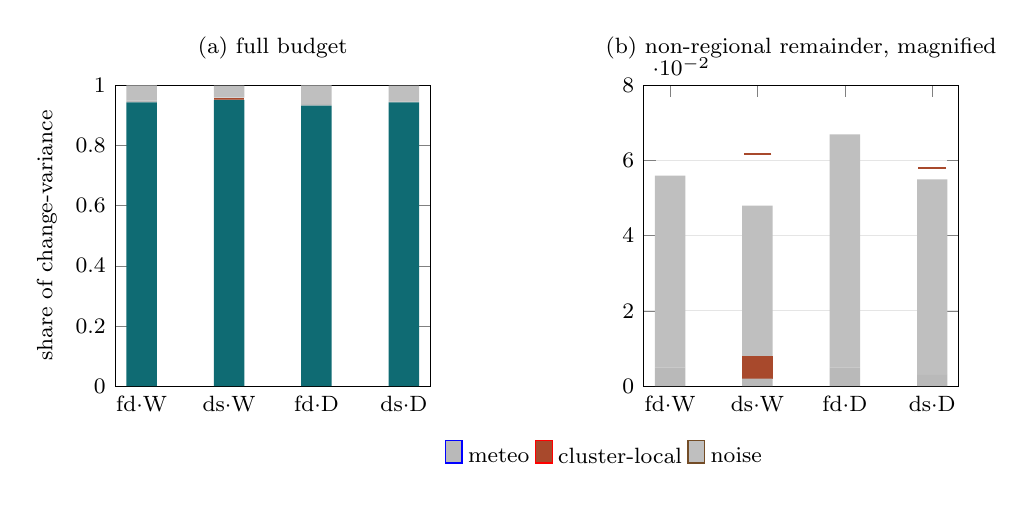
\begin{tikzpicture}
\begin{axis}[
  name=vfull,
  width=0.46\linewidth, height=5.4cm,
  ybar stacked, bar width=11pt,
  ymin=0, ymax=1,
  ylabel={share of change-variance},
  title={\footnotesize (a) full budget},
  symbolic x coords={fd$\cdot$W, ds$\cdot$W, fd$\cdot$D, ds$\cdot$D},
  xtick=data,
  tick label style={font=\footnotesize},
  label style={font=\footnotesize},
  every axis plot/.append style={draw=none},
]
\addplot+[fill=noxink] coordinates {(fd$\cdot$W,0.944)(ds$\cdot$W,0.951)(fd$\cdot$D,0.933)(ds$\cdot$D,0.944)};
\addplot+[fill=gray!55]  coordinates {(fd$\cdot$W,0.005)(ds$\cdot$W,0.002)(fd$\cdot$D,0.005)(ds$\cdot$D,0.003)};
\addplot+[fill=noxember] coordinates {(fd$\cdot$W,0.000)(ds$\cdot$W,0.006)(fd$\cdot$D,0.000)(ds$\cdot$D,0.000)};
\addplot+[fill=black!25]  coordinates {(fd$\cdot$W,0.051)(ds$\cdot$W,0.040)(fd$\cdot$D,0.062)(ds$\cdot$D,0.052)};
\end{axis}
% Panel (b): the same non-regional remainder on an axis that can actually resolve it.
\begin{axis}[
  name=vzoom, at=(vfull.right of south east), anchor=left of south west,
  width=0.46\linewidth, height=5.4cm,
  ybar stacked, bar width=11pt,
  ymin=0, ymax=0.08,
  ylabel={}, title={\footnotesize (b) non-regional remainder, magnified},
  symbolic x coords={fd$\cdot$W, ds$\cdot$W, fd$\cdot$D, ds$\cdot$D},
  xtick=data,
  legend style={at={(-0.12,-0.16)},anchor=north,draw=none,font=\footnotesize,legend columns=3},
  tick label style={font=\footnotesize},
  label style={font=\footnotesize},
  ymajorgrids, grid style={gray!20},
  every axis plot/.append style={draw=none},
]
\addplot+[fill=gray!55]  coordinates {(fd$\cdot$W,0.005)(ds$\cdot$W,0.002)(fd$\cdot$D,0.005)(ds$\cdot$D,0.003)};
\addplot+[fill=noxember] coordinates {(fd$\cdot$W,0.000)(ds$\cdot$W,0.006)(fd$\cdot$D,0.000)(ds$\cdot$D,0.000)};
\addplot+[fill=black!25]  coordinates {(fd$\cdot$W,0.051)(ds$\cdot$W,0.040)(fd$\cdot$D,0.062)(ds$\cdot$D,0.052)};
\legend{meteo, cluster-local, noise}
% Upper 95% bootstrap bound on the cluster-local share, the quantity the null actually excludes.
\addplot[only marks, mark=-, mark size=5pt, thick, noxember, forget plot]
  coordinates {(fd$\cdot$W,0.0000)(ds$\cdot$W,0.0138)(fd$\cdot$D,0.0000)(ds$\cdot$D,0.0030)};
\end{axis}
\end{tikzpicture}
\caption{Change-variance budget per cell (W: weekly, D: daily; fd: first-difference, ds:
deseasonalised). (a) The regional common mode fills the bar, which is the finding but also makes
everything else unreadable. (b) The same bars with the regional term removed and the axis
magnified $12.5\times$, so the terms that are actually in contention can be seen: the
cluster-local slice (ember) is a hairline against noise, and in three of four cells its raw
incremental $R^2$ is slightly \emph{negative} (Table~\ref{tab:variance}). Ember tick marks in (b)
are the upper 95\% moving-block bootstrap bounds on the cluster-local share --- the quantity the
null excludes rather than the point estimate it reports, at most $0.014$ (weekly deseason) and
indistinguishable from zero elsewhere. All values are at the 25--60\,km ring;
Section~\ref{sec:ringsweep} shows they move with it.}
\label{fig:variance}
\end{figure}

Three of the four cells return a small negative raw $\Delta R^2_{\text{local}}$
($-0.021$, $-0.026$, $-0.0003$); the fourth returns $+0.006$. A negative incremental $R^2$ in a
nested partition of this form means the local term buys nothing and its inclusion costs degrees
of freedom --- the cluster-local component is statistically indistinguishable from zero, and if
anything the point estimate sits marginally on the wrong side of it. We report the raw values
rather than only the clamped share because the clamping is otherwise invisible, and a table that
shows a clean $0.000$ without saying it was clamped misrepresents the estimate.

The measured cluster-local change-variance share is thus $\approx0$ \emph{at this ring geometry}:
the footprint and the 25--60\,km ring move nearly in lockstep at both weekly and daily cadence. The
hypothesis that a change detector has variance-share headroom over a level estimator is not
supported at 25--60\,km.

\paragraph{But the share is ring-dependent, and we now know it.} The qualifier in the preceding
sentence is not decorative. Section~\ref{sec:ringsweep} reports a sensitivity sweep of the ring
radii out to 90--150\,km: the cluster-local share is \emph{not} stable across ring geometries, and
on one of the two change bases it rises by a factor of $8.7$ as the ring moves outward --- without
plateauing --- with a bootstrap confidence interval that excludes zero from 40--80\,km onward. The $\approx0$ in Table~\ref{tab:variance} is
therefore a property of the footprint-minus-25--60\,km-ring contrast, not a scale-free property of
the cluster, and we no longer present it as one.

\subsection{Two ways this result could be an artefact of its own geometry}
\label{sec:ringcaveat}

The result in Section~\ref{sec:variance} is the load-bearing one for this paper, so we state its
two most serious alternative explanations explicitly. We were subsequently able to test the first
and not the second; neither is excluded.

\paragraph{(i) The background ring may contain the cluster's own plume.} The flux analysis
(Section~\ref{sec:flux}) measures a mean effective wind of $|U|=2.48$\,m\,s$^{-1}$ over the AOI
and assumes a \ce{NO_2} lifetime $\tau=4$\,h. The implied advection length is
$|U|\tau\approx36$\,km --- which lands near the middle of the 25--60\,km background ring
(Fig.~\ref{fig:map}). If a material part of the cluster's emitted \ce{NO_2} is present in the
ring as advected plume, then subtracting the ring subtracts part of the signal along with the
background, and the fixed regional\,$\to$\,meteo\,$\to$\,local partition order
(Section~\ref{sec:methods}) then books that shared variance to the ``regional'' term by
construction. A cluster-local share of $\approx0$ is exactly what ring self-subtraction would
also produce. We ran the discriminating sweep; Section~\ref{sec:ringsweep} reports it.

\paragraph{(ii) Part of the ``regional common mode'' may be retrieval artefact rather than
atmosphere.} A 93--95\% common mode between the footprint and its surrounding ring is a large
number, and the TROPOMI retrieval supplies at least two mechanisms that would produce one without
any atmospheric coherence. The stratosphere--troposphere separation subtracts a stratospheric
field that is smoothed to roughly $1\degree$, and the air-mass factor uses a priori \ce{NO_2}
profiles from the TM5 chemistry-transport model at coarse resolution. Both fields are, by
construction, spatially smooth across an AOI and a ring that together span well under
$2\degree$. Any residual error in either therefore appears as a common additive or multiplicative
term shared almost perfectly between footprint and ring, and inflates the measured common-mode
share mechanically.

We have not quantified this contribution, and it cannot be quantified from the level-3 composited
product we use: separating it requires the per-overpass stratospheric column and AMF fields,
propagated through the same compositing. The honest statement is that 0.93--0.95 is an upper
bound on the \emph{atmospheric} common mode, not an estimate of it. This does not overturn the
paper's conclusion --- a cluster signal that cannot be separated from a retrieval-borne common
mode is just as unrecoverable in practice as one buried in a real regional plume --- but it does
change the physical interpretation, and a reviewer is entitled to that distinction.

\subsection{Ring-radius sensitivity: the cluster-local share is ring-dependent}
\label{sec:ringsweep}

The concern in Section~\ref{sec:ringcaveat}(i) is testable, so we tested it --- twice. Holding the
decomposition, the change bases, the cadences, the partition order, the covariates, the seed and
the bootstrap depth all fixed, we swept only the background ring's radii. The decision rules were
fixed before each run.

\paragraph{The first sweep was geometry-limited, and we say so.} Run on the AOI of
Section~\ref{sec:data} (facility bbox $+\,0.25\degree$), it reached 60--120\,km and returned
\emph{inconclusive}. That AOI, however, extends only 63\,km from the cluster centroid with full
$360\degree$ coverage; past that radius its rectangle contributes four corner wedges, not an
annulus, and the outermost ring the run could form was truncated at $\approx124$\,km. Equal-octant
weighting attenuates such anisotropy but cannot manufacture the missing azimuths. We therefore
re-acquired the whole TROPOMI record over a $1.25\degree$ buffer --- $4.8\times$ the area,
2{,}741 overpasses, a $66\times109$ grid at the identical $0.055\degree\times0.035\degree$ step
--- and re-ran the same sweep out to 90--150\,km. All seven rings in
Table~\ref{tab:ringsweep} are complete annuli: all eight octants populated, realised outer radius
within 0.03\,km of the requested one.

\paragraph{The two cubes agree where they overlap.} The wide grid's step matches but its origin is
offset by a fraction of a cell, so the footprint discretises to 447 cells rather than 448 and the
ERA5 footprint means shift by ${\le}0.05$\,m\,s$^{-1}$. Rather than assume that immaterial, we
re-ran the \emph{committed} 25--60\,km ring on the wide cube truncated to the original record's end.
Every share agrees to within $0.0035$ and every sample size to within 2 observations. The
period-retention audit is likewise clean: the wide cube's retained weeks are a strict superset of
the committed cube's ($0$ weeks lost, 11 gained, all in the tail added by the later download),
because the period-coverage mask was evaluated over the original $0.25\degree$ sub-box precisely so
that $n$ could not move at the same time as the ring.

\begin{table}[t]
\centering
\caption{Cluster-local (and, in parentheses, regional) change-variance share by background-ring
radius on the $1.25\degree$ cube, plain ring weighting. Only the ring varies; every other parameter
is held at its Section~\ref{sec:variance} value. Every ring is a complete annulus (eight octants
populated). The first-difference basis reports a clamped zero at \emph{every} radius. Weekly
$n=389$ (deseason) / 388 (first-difference); daily $n=2{,}001$ / 1{,}556.}
\label{tab:ringsweep}
\small
\begin{tabular}{@{}lrrrr@{}}
\toprule
Ring (km) & cells & deseason\,$\cdot$\,W & deseason\,$\cdot$\,D & first-diff (W \& D) \\
\midrule
25--60  &  293 & 0.007 \; (0.954) & 0.000 \; (0.946) & 0.000 \; (0.947 / 0.935) \\
40--80  &  575 & 0.009 \; (0.936) & 0.000 \; (0.942) & 0.000 \; (0.927 / 0.931) \\
50--90  &  752 & 0.016 \; (0.911) & 0.001 \; (0.926) & 0.000 \; (0.903 / 0.914) \\
60--100 &  970 & 0.026 \; (0.884) & 0.004 \; (0.907) & 0.000 \; (0.884 / 0.896) \\
60--120 & 1{,}737 & 0.036 \; (0.854) & 0.008 \; (0.883) & 0.000 \; (0.863 / 0.872) \\
75--135 & 2{,}152 & 0.049 \; (0.805) & 0.014 \; (0.839) & 0.000 \; (0.821 / 0.831) \\
90--150 & 2{,}514 & \textbf{0.061} \; (0.758) & \textbf{0.023} \; (0.793) & 0.000 \; (0.781 / 0.788) \\
\bottomrule
\end{tabular}
\end{table}

\begin{figure}[t]
\centering
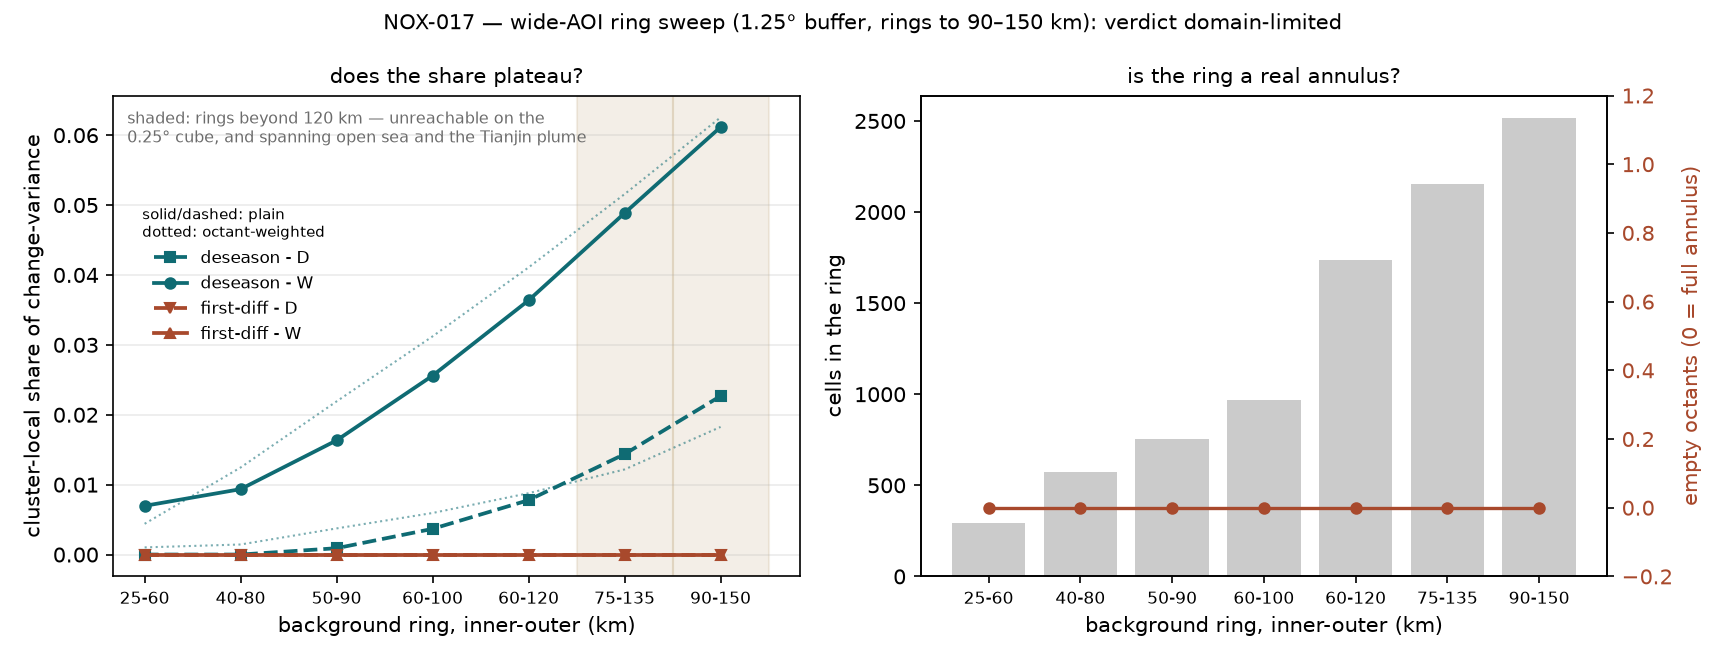
\includegraphics[width=\linewidth]{figures/wide_ring_sensitivity.png}
\caption{Left: cluster-local change-variance share against ring geometry on the $1.25\degree$ cube;
dotted lines are the equal-octant-weighted variant. The shaded band marks the rings the
$0.25\degree$ AOI could not form. The deseason basis rises monotonically and is still rising at the
outermost ring; the first-difference basis does not move at all. Right: the geometry audit --- ring
size grows from 293 to 2{,}514 cells while the count of empty octants stays at zero, so every ring
is a genuine annulus rather than a set of corner wedges.}
\label{fig:ringsweep}
\end{figure}

\paragraph{Widening the domain did not make the share converge.} On the deseasonalised basis the
cluster-local share rises monotonically with ring radius --- weekly $0.007\to0.061$, a factor of
$8.7$; daily $0.000\to0.023$ --- and its moving-block bootstrap interval excludes zero from the
40--80\,km ring outward (weekly lower bound $0.001\to0.023$). The regional share falls from
$0.95$ to $0.76$ over the same sweep, and it falls on the first-difference basis too
($0.947\to0.781$). At the outermost ring the weekly deseason cell clears, for the first time, both
pre-registered materiality thresholds: its level ($0.061$) and its rise from the baseline ring
($+0.054$) each exceed $0.05$.

Against that, three things. The quorum is not met --- both rules require two of the four
(basis\,$\times$\,cadence) cells and only one fires. The first-difference basis is a clamped zero at
\emph{every} radius, so the variance leaving the regional term on that basis goes to meteorology and
noise rather than to the cluster; a ring that were simply eating the cluster's plume should hand
variance back to both bases once it moves away. And the share has \emph{not} plateaued: the last
increment is $+0.012$ weekly against a pre-registered plateau tolerance of $0.01$. The sweep's own
rule therefore returns \textbf{domain-limited}.

\paragraph{What we can and cannot now say.} Self-subtraction is \emph{not} established.
Ring-robustness is not established either, and that is the change that matters: the $\approx0$ of
Section~\ref{sec:variance} is demonstrably a property of the footprint-minus-25--60\,km-ring
contrast rather than of the cluster, and by 90--150\,km the cluster-local share is an order of
magnitude larger and no longer statistically indistinguishable from zero. The new information over
the first sweep is negative and worth stating plainly: quadrupling the AOI area and pushing the
ring to 150\,km did not produce convergence. The ring radius is not a parameter that settles down
over any domain this cluster's geography allows, so the share must be quoted as a range across ring
geometries rather than at any single radius.

One limit is now unavoidable rather than incidental. At 90--150\,km the background ring spans the
Bohai Sea and the Tianjin urban plume: it is no longer the same air mass as the cluster. A share
that keeps rising at that radius may be responding to a change of air mass rather than to escaping
the cluster's own plume, and no sweep of this design can separate the two. Pushing the ring further
would make that confound worse, not better --- which is why we stop here and report the result as
domain-limited rather than acquiring a wider cube again.

\subsection{A wider-scale benchmark does not rescue the signal either}
\label{sec:scalecontrast}

Section~\ref{sec:limitations} of an earlier draft listed, as its second missing control, the cheap
test that discriminates between the two explanations for the near-null: does the \emph{same}
feature track \emph{wider-scale} steel activity? If a Tangshan-AOI \ce{NO_2} feature tracks national
steel better than it tracks Tangshan's own BF rate, the AOI column is carrying a regionally
coherent component --- the paper's spatial reading --- and the feature is measuring something real
about steel. We ran it (Table~\ref{tab:scalecontrast}).

\begin{table}[t]
\centering
\caption{Scale contrast, full record, benchmark-blind features scored unchanged against targets
ordered by spatial scale. All four targets are shown; the appendix (Table~\ref{tab:scalecontrast-full})
reports the complete family of 24 pairings including the two sub-period splits, over which the
BH-FDR correction is computed. ``Contrast'' is the paired difference $r(\text{target}) -
r(\text{Tangshan})$ with a moving-block bootstrap CI on the \emph{common} sample --- not two
marginal intervals compared by eye; $\dagger$ marks a contrast whose CI excludes zero.
\emph{No pairing is robust-significant after FDR correction.}}
\label{tab:scalecontrast}
\small
\begin{tabular}{@{}llcrrrr@{}}
\toprule
Feature & Target (scale) & cad. & $n$ & $r$ & BH $p$ & contrast vs Tangshan [95\% CI] \\
\midrule
intensity & Tangshan BF (cluster) & W & 379 & $+0.062$ & 0.466 & --- (baseline) \\
intensity & national BF rate & W & 382 & $-0.094$ & 0.366 & $-0.165\;[-0.300,-0.018]$$^{\dagger}$ \\
intensity & national crude steel & ME & 89 & $-0.222$ & 0.366 & $-0.360\;[-0.647,+0.034]$ \\
intensity & national pig iron & ME & 89 & $-0.154$ & 0.419 & $-0.292\;[-0.532,+0.055]$ \\
\addlinespace
residual & Tangshan BF (cluster) & W & 364 & $-0.014$ & 0.864 & --- (baseline) \\
residual & national BF rate & W & 367 & $-0.090$ & 0.366 & $-0.082\;[-0.233,+0.079]$ \\
residual & national crude steel & ME & 89 & $-0.120$ & 0.523 & $-0.103\;[-0.446,+0.379]$ \\
residual & national pig iron & ME & 89 & $-0.110$ & 0.554 & $-0.093\;[-0.376,+0.333]$ \\
\bottomrule
\end{tabular}
\end{table}

\textbf{Widening the target does not strengthen the coupling.} The national pairings are near-null
too, and the paired contrast is negative throughout --- the national targets are tracked, if
anything, slightly worse than Tangshan's own. Under the pre-registered rule the outcome is
\emph{pipeline-suspect}: no national pairing reaches $|r|=0.20$ on the primary target (best
$0.094$), far below the $0.5$--$0.75$ range the national-scale nowcasting literature reports.

One contrast is worth stating rather than absorbing into the summary. For the intensity feature
against the national BF rate the paired difference is $-0.165\;[-0.300,-0.018]$, and that interval
\emph{excludes zero}: the national target is tracked measurably \emph{worse} than Tangshan's own,
not merely no better. The direction is the opposite of what the spatial reading predicts --- a
Tangshan column dominated by a regionally coherent component should proxy the wider aggregate at
least as well as the local one. We do not over-read a single contrast in a family of 24 whose FDR
correction leaves nothing significant, but describing the family as uniformly null would omit its
one directional result, and that result runs against our own interpretation.

The complete family, including the two sub-period splits, is in
Table~\ref{tab:scalecontrast-full}. We report all 24 rather than the eight full-record rows
because three of the hidden cells reach nominal significance on the block-permutation test
(intensity\,$\times$\,national crude steel, 2019--2021, \rval{-0.392}, $p=0.036$;
residual\,$\times$\,national pig iron, 2022--2026, \rval{+0.306}, $p=0.037$;
intensity\,$\times$\,national pig iron, 2019--2021, \rval{-0.365}, $p=0.059$), and all three die
under the family-wide correction. Showing only the rows that agree with the summary, while
computing the correction over rows the reader cannot see, would be the same scan-selection error
that Section~\ref{sec:regime} exists to diagnose.

\paragraph{Read this carefully in both directions.} It does \emph{not} establish that the pipeline
is broken. Our feature is a Tangshan-AOI window --- $\sim$13\% of national steel, under
$2\degree$ across --- not national-coverage \ce{NO_2}, so it was never guaranteed to proxy national
output; the decisive form of that test needs a province- or nation-scale cube, which we did not
build. Nor does it break the feature-versus-target ambiguity: all four targets are CREA/WIND
survey products, so a survey-methodology artefact would move them together. The arm that would have
added an independent publisher --- NBS provincial and national monthly crude steel --- was gated on
a live feasibility probe, and the probe returned NO-GO: every NBS data endpoint refuses
programmatic access, while static assets on the same host serve normally. Per our free-data rule we
did not substitute a paywalled provider, so that gap stays open.

What it \emph{does} establish is narrower and still consequential: the cheap test that would have
corroborated the spatial explanation was run, and it did not corroborate it. We note also that the
national correlations are strongly sub-period dependent ($-0.34$ to $-0.39$ over 2019--2021,
collapsing toward zero over 2022--2026), which is inseparable from the unharmonised
processor-version sequence of Section~\ref{sec:data}.

\subsection{The public thermal proxy is uninformative here}
\label{sec:viirs}

To break the feature-versus-target ambiguity we sought a proxy that no statistical office can
adjust: a space-based thermal signature over the facilities. The product tuned for sub-pixel
high-temperature industrial sources (VIIRS Nightfire) is licence/pay-gated and thus outside a
free-data scope; the free active-fire archive was therefore acquired in full and triangulated,
blind to the benchmark, against both \ce{NO_2} and the CREA rate (Table~\ref{tab:viirs}).

\begin{table}[t]
\centering
\caption{Thermal triangulation, weekly, $n=373$ (autocorrelation-robust). The fire signal tracks
neither series, so it cannot arbitrate feature versus target.}
\label{tab:viirs}
\small
\begin{tabular}{lrrrrl}
\toprule
Pairing & $r$ (lag 0) & $p$ (Newey--West) & $p$ (perm) & BH $p_{\text{adj}}$ & read \\
\midrule
\ce{NO_2} $\leftrightarrow$ fire & $-0.054$ & 0.343 & 0.336 & 0.630 & not significant \\
CREA $\leftrightarrow$ fire      & $-0.049$ & 0.612 & ---   & 0.630 & not significant \\
\bottomrule
\end{tabular}
\end{table}

The cause is physical: active-fire detections over this AOI are dominated by seasonal
agricultural crop-residue burning --- the detection climatology peaks in spring--autumn and is
$\approx0$ in winter (normalised: Jan 0.00, May 0.87, Sep 1.00, Dec 0.09) with low radiative
power ($\sim$1.4\,MW median), a shape that persists even within 2\,km of the facilities. Blast
furnaces run year-round and are winter-\emph{curtailed}, so a genuine furnace thermometer would
peak in winter. The active-fire product does not detect the furnaces; the product that could
(Nightfire) is behind a paywall. This is an informative proxy-validity result, not a claim that
\ce{NO_2} is weak.

\paragraph{The benchmark is not the weak link, and this is measurable.} The thermal route was
meant to arbitrate feature against target and could not. A cheaper bound is available and we
report it, because ``perhaps the trader survey is simply noisy'' would otherwise remain an
unexamined escape from every result in this paper. CREA publishes, in the same release, a
separately surveyed national panel --- the blast-furnace starting rate across 247 mills. Over the
study window the Tangshan rate tracks that panel at \rval{+0.76} in weekly \emph{changes}
($n=376$, moving-block bootstrap 95\% CI $[+0.51,+0.85]$), and at \rval{+0.26} in levels. A series
whose week-to-week movement is $76\%$ correlated with an independently surveyed national panel is
not dominated by survey noise. Under the usual attenuation argument its reliability is bounded
below by that figure, so measurement error in the target caps the attainable correlation at
$\sqrt{0.76}\approx0.87$ --- an order of magnitude above the $0.17$ this study excludes
(Table~\ref{tab:equivalence}). The near-null cannot be explained by a noisy benchmark.

We are careful about what this does not do. Both series are published by CREA from WIND inputs, so
this bounds the target's \emph{reliability} --- its reproducibility as a measurement --- and not
its \emph{validity}: a shared survey-methodology artefact would move the Tangshan and national
panels together and be invisible to this test. Closing that gap needs an independent publisher,
which Section~\ref{sec:scalecontrast} reports was gated on a probe that returned NO-GO. What the
test removes is the specific and otherwise untestable objection that the benchmark carries too
little signal to correlate with anything.

\subsection{The continuous coupling is near-null; the 2023 peak is a scan-maximum artefact}
\label{sec:regime}

Exploratory analysis surfaced one encouraging pattern: a rolling correlation peaking in mid-2023.
A rolling-window maximum is, however, a multiple-comparisons statistic. We tested it with fixed,
benchmark-blind parameters and a scan-maximum null --- a serial-dependence-preserving block
permutation whose reference distribution is the maximum rolling-$r$ over all 341 overlapping
78-week windows. The peak is \rval{0.276} (2023-08-27) and sits at the \textbf{67.5th percentile}
of its own scan-maximum null ($p=0.325$): entirely unremarkable given how many windows were
scanned.

\paragraph{Two correlations that must not be confused.} Within the 78-week window that produced
the peak, the intensity residual correlates with the benchmark at \rval{0.257} ($n=78$; the small
difference from the $0.276$ rolling value is the weekly re-alignment used by the jackknife
routine). Over the \emph{full record}, the same residual correlates with the same benchmark at
\rval{+0.063} ($n=379$; Table~\ref{tab:nowcast}). These are not in conflict, and the $0.257$ is
not a full-record figure: it is the correlation inside the window that was selected \emph{because}
it maximised the correlation. Reporting it without that qualification --- as an earlier draft of
this paper did --- would be the scan-maximum error the section exists to diagnose. The full-record
value is the one that describes the coupling; the within-peak value describes the selection.

\paragraph{The jackknife rules out one alternative, not much more.} A leave-one-event-out
jackknife within the peak window removes the observations lying within $\pm4$ weeks of each of the
21 sourced curtailment events, and re-measures. Removing the three highest-contribution events
moves the within-window $r$ from $0.257$ to $0.349$. We read this narrowly: no single curtailment
event carries the peak, so the peak is not a one-event artefact. We do \emph{not} read it as
evidence of continuous coupling. Removing three events with a $\pm4$-week exclusion drops roughly
27 of 78 observations, so the $0.349$ is measured on $n\approx51$ within an already
scan-selected window; no significance is attached to it, and the change from $0.257$ is well
inside the sampling variability of a correlation on that many points. That the correlation
\emph{rises} when the largest curtailment events --- the periods where a genuine
activity$\to$\ce{NO_2} response should be most visible --- are removed is, if anything, evidence
against a physical curtailment response and is not a result we can explain. The controlling number
remains the full-record $+0.063$.

\paragraph{2024.} The dual collapse diagnostic attributes the post-2023 fall-off to an intensity
shift rather than a change in the curtailment calendar. Given Section~\ref{sec:baseline}, we no
longer interpret that intensity shift physically: a slow change in the \ce{NO_2}-per-unit-output
ratio is not separable from processor-version drift in this record.

\subsection{No forecasting skill over the operational benchmark}
\label{sec:nowcast}

We next ask whether a public-data \ce{NO_2} nowcast can improve on the operational CREA
benchmark. A screen measured, blind to the benchmark and at fixed parameters, whether any
available \ce{NO_2} feature carries incremental information over the benchmark. The valid-proxy
route is closed (Section~\ref{sec:viirs}), and neither \ce{NO_2} feature clears the bar
(Table~\ref{tab:nowcast}).

\begin{table}[t]
\centering
\caption{Forecasting-skill screen, weekly, blind to the benchmark. Both permutation $p$-values are
far from significance and both bootstrap CIs straddle zero. The cross-correlation peaks are
reported for completeness only: neither exceeds its own per-lag significance bound, and the
first sits at $-8$ weeks, the edge of the scanned $\pm8$-week window, so it is a boundary
selection and not an estimated lag. No lead or lag is identified by these data.}
\label{tab:nowcast}
\small
\begin{tabular}{@{}lrrrcrr@{}}
\toprule
\ce{NO_2} feature & $n$ & $r$ (0) & $p$ (perm) & boot 95\% CI & peak lag\,/\,$r$ & bound \\
\midrule
Background-corrected residual & 364 & $-0.014$ & 0.815 & $[-0.120,+0.081]$ & $-8$\,wk\,/\,$-0.085$ & $\pm0.103$ \\
Intensity-decomp.\ covariate & 379 & $+0.063$ & 0.290 & $[-0.049,+0.157]$ & $-2$\,wk\,/\,$+0.082$ & $\pm0.101$ \\
\bottomrule
\end{tabular}
\end{table}

Both peak $|r|$ values fall below their per-lag white-noise bounds ($0.085<0.103$;
$0.082<0.101$), before any correction for having scanned 17 lags. An earlier draft of this paper
described these peaks as showing that ``the feature follows the benchmark rather than leading
it''. That claim is withdrawn: it reads structure into two non-significant statistics, one of
which is pinned to the boundary of the scan window, and it is precisely the error that
Section~\ref{sec:regime} is devoted to identifying elsewhere. The correct statement is that no
lead--lag structure is detectable at all.

The screen is negative, so the fuller feature/baseline/surprise model it would have justified was
not built. This is the expected consequence of Section~\ref{sec:variance}: a residual dominated
by the regional common mode cannot lead a cluster-activity benchmark.

\paragraph{A parallel market screen, reported in full.} We also asked whether \ce{NO_2}-derived
event markers anticipate steel-sector equity moves. The detector flags 27 \ce{NO_2} events
(16 surge, 11 drop) over 2019--2026; forward cumulative abnormal returns (CAR) were measured over
a 5-day window against a global market index (ACWI), with the first tradeable session set at
overpass $+2$ days so no look-ahead is possible (Table~\ref{tab:market}).

\begin{table}[t]
\centering
\caption{Market event study on \ce{NO_2}-detected production events ($n=27$ events per
instrument): 5-day forward cumulative abnormal return relative to ACWI, with a
bootstrap 95\% CI, and the fraction of events with positive CAR. All four CIs contain zero and
all hit rates are within sampling range of $0.5$. The 108 event$\times$instrument tests are
\emph{not} multiplicity-adjusted, so these are exploratory by construction. The upstream event
detector is itself weak (4/47 production events matched; precision 0.15, recall 0.09).}
\label{tab:market}
\small
\begin{tabular}{llrcr}
\toprule
Instrument & Exposure & CAR (5\,d) & boot 95\% CI & hit rate \\
\midrule
BHP  & diversified miner        & $+0.0008$ & $[-0.0136,+0.0120]$ & 0.48 \\
RIO  & diversified miner        & $+0.0044$ & $[-0.0074,+0.0140]$ & 0.41 \\
VALE & iron-ore producer        & $-0.0020$ & $[-0.0227,+0.0157]$ & 0.48 \\
SLX  & steel-sector ETF         & $-0.0079$ & $[-0.0217,+0.0041]$ & 0.41 \\
\bottomrule
\end{tabular}
\end{table}

No tradable \ce{NO_2}$\rightarrow$market link is present in these data. We report the table rather
than the one-line summary an earlier draft carried, because a claim of this kind with no $n$, no
statistic and no method is not checkable and should not be made.

\subsection{Flux divergence detects no separable source at the depth we could reach}
\label{sec:flux}

The remaining route attacks the regional background directly: \ce{NO_2} \emph{flux divergence}
\citep{beirle_2021,beirle_2023}. One forms the horizontal flux $\mathbf{F}=\Omega\,\mathbf{w}$
(column $\Omega$ times ERA5 wind $\mathbf{w}$) and takes its divergence
$\nabla\!\cdot\!\mathbf{F}$, which isolates the local source term and should separate a Tangshan
source from the advected background. Averaging many overpasses (each with its own wind, so
advection dipoles cancel) should drive field noise down $\sim\!1/\sqrt{N}$. The decisive question
is whether the co-located source \emph{separates} --- SNR climbing toward the detection
thresholds --- or stays flat as the noise falls (Table~\ref{tab:flux}, Fig.~\ref{fig:snr}). The
pipeline fixes two such thresholds in advance: $\mathrm{SNR}\ge3.0$ for a clean detection
(\texttt{snr\_go}) and $\ge1.5$ for a partial-but-usable one (\texttt{snr\_degraded}). Both are
compiled-in constants, set before any real swath was processed. Figures below are referenced
against the \emph{lower} of the two, which is the more generous test.

\begin{table}[t]
\centering
\caption{Multi-overpass scaling (real Level-2 swaths, blind to the benchmark). Noise is the median
absolute deviation of the background divergence field (mol\,m$^{-2}$\,s$^{-1}$). The last two
columns are references, not fits: the $1/\sqrt{N}$ noise expectation from $N{=}1$, and the SNR a
constant source term would produce if the noise fell as $1/\sqrt{N}$ from the $N{=}1$ value.
There is one realisation per row, so no uncertainty is attached to any entry.}
\label{tab:flux}
\small
\begin{tabular}{@{}rrrrrr@{}}
\toprule
$N$ & SNR & co-location ratio & noise (MAD) & $1/\sqrt{N}$ noise ref. & SNR if source constant \\
\midrule
1 & $+0.27$ & 2.06 & $3.618\times10^{-8}$ & $3.618\times10^{-8}$ & $+0.27$ \\
2 & $+0.22$ & 2.29 & $1.770\times10^{-8}$ & $2.558\times10^{-8}$ & $+0.38$ \\
4 & $+0.27$ & 1.80 & $1.068\times10^{-8}$ & $1.809\times10^{-8}$ & $+0.54$ \\
\bottomrule
\end{tabular}
\end{table}

\begin{figure}[t]
\centering
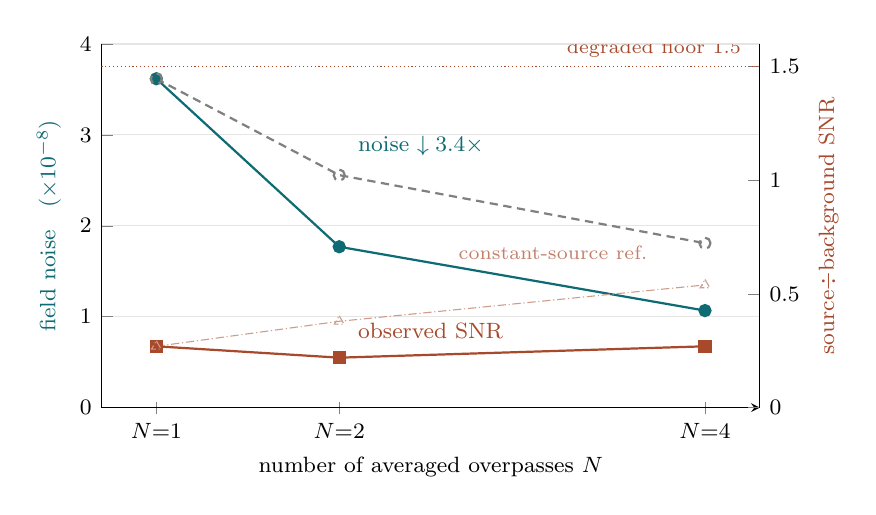
\begin{tikzpicture}
\begin{axis}[
  name=main,
  width=0.82\linewidth, height=6.2cm,
  axis y line*=left, axis x line=bottom,
  xlabel={number of averaged overpasses $N$},
  ylabel={\textcolor{noxink}{field noise \; $(\times10^{-8})$}},
  xmin=0.7, xmax=4.3, ymin=0, ymax=4,
  xtick={1,2,4}, xticklabels={$N{=}1$,$N{=}2$,$N{=}4$},
  tick label style={font=\footnotesize}, label style={font=\footnotesize},
  ymajorgrids, grid style={gray!20},
]
\addplot[noxink, thick, mark=*, mark options={fill=noxink}]
  coordinates {(1,3.618)(2,1.770)(4,1.068)};
\addplot[gray, densely dashed, thick, mark=o]
  coordinates {(1,3.618)(2,2.558)(4,1.809)};
\end{axis}
\begin{axis}[
  width=0.82\linewidth, height=6.2cm,
  at=(main.south east), anchor=south east,
  axis y line*=right, axis x line=none,
  ylabel={\textcolor{noxember}{source$\div$background SNR}},
  xmin=0.7, xmax=4.3, ymin=0, ymax=1.6,
  tick label style={font=\footnotesize}, label style={font=\footnotesize},
]
\addplot[noxember, densely dotted] coordinates {(0.7,1.5)(4.3,1.5)};
\addplot[noxember, thick, mark=square*, mark options={fill=noxember}]
  coordinates {(1,0.27)(2,0.22)(4,0.27)};
\addplot[noxember!55, densely dashdotted, mark=triangle]
  coordinates {(1,0.27)(2,0.38)(4,0.54)};
\node[font=\footnotesize, noxink,  anchor=west] at (axis cs:2.05,1.15) {noise $\downarrow3.4\times$};
\node[font=\footnotesize, noxember,anchor=west] at (axis cs:2.05,0.34) {observed SNR};
\node[font=\scriptsize, noxember!70,anchor=west] at (axis cs:2.6,0.68) {constant-source ref.};
\node[font=\scriptsize, noxember,anchor=east] at (axis cs:4.25,1.58) {degraded floor 1.5};
\end{axis}
\end{tikzpicture}
\caption{Signal-to-noise ratio versus averaging depth $N$ over the four real overpasses obtained.
Field noise (teal, left axis) falls $3.4\times$ from $N{=}1$ to $N{=}4$, which is
\emph{faster} than the $1/\sqrt{N}$ reference (grey dashed) --- see the text: this is not the
confirmation of theory it may appear to be. The observed SNR (solid ember, right axis) stays near
$+0.27$, well below both the 1.5 degraded-detection floor and the dash-dotted reference showing where the
SNR would sit if a constant source term were divided by an ideal $1/\sqrt{N}$ noise. Three points,
one realisation each, no error bars: the figure is a description, not a test.}
\label{fig:snr}
\end{figure}

\paragraph{What the numbers show.} High \ce{NO_2} remains co-located with the plants (ratio
1.8--2.3$\times$), but that is expected --- the plants sit in the cluster's \ce{NO_2} core --- and
flux divergence does not convert co-location into a separable \emph{source} here. The footprint
source-term median ($8.15\times10^{-9}$\,mol\,m$^{-2}$\,s$^{-1}$) sits near the background level
($5.31\times10^{-9}$), both far below the $N{=}4$ noise ($1.07\times10^{-8}$). The observed SNR
at $N{=}4$ is $0.27$ against the $0.54$ that a constant source term over ideally averaging noise
would give, so the numerator is falling roughly in step with the denominator.

\paragraph{Why $N{=}4$ does not license a strong claim.} We reached four overpasses of an intended
ten to twelve; the CDSE zipper endpoint throttled sustained pulls to $\sim$1.6\,MB\,s$^{-1}$, and
the access API offers no server-side spatial subsetting, so a full-record inversion means
$\sim$2.3\,TB of transfer. Four is two to three orders of magnitude below the operating point of
the method we are applying: the published TROPOMI point-source catalogues are built from two to
three years of near-daily coverage, i.e.\ of order $10^2$--$10^3$ usable overpasses per location
\citep{beirle_2021,beirle_2023}. The throttling explains why we stopped at four; it does not make
four sufficient.

We had previously offered a scaling extrapolation --- ``if SNR grows as $\sqrt{N}$, lifting $0.27$
to the floor needs $N\approx124$ from $N{=}4$, or $N\approx31$ from $N{=}1$'' --- as an
acquisition estimate. It is withdrawn as such, for two reasons. First, the two figures are
mutually inconsistent under a single model, which is the signature of an extrapolation whose
premise does not hold: $\sqrt{N}$ growth from $N{=}1$ predicts $\mathrm{SNR}(4)=0.54$, and the
measured value is $0.27$. The data in Table~\ref{tab:flux} therefore \emph{falsify} the premise of
the extrapolation over the only range in which we can check it. Second, the target is misstated.
The $1.5$ threshold is the pipeline's \texttt{snr\_degraded} level --- ``partial but usable'' ---
whereas a clean detection is defined at \texttt{snr\_go}~$=3.0$; reaching that from $0.27$ under
the same (falsified) $\sqrt{N}$ assumption would need $N\approx494$. The defensible statement is
conditional and we leave it in that form: \emph{if} the flat SNR over $N=1$--$4$ is sampling noise
around a genuine $\sqrt{N}$ growth, then order $10^2$ overpasses would be required to reach even
the degraded threshold; if it is not, no achievable $N$ helps. Four overpasses cannot distinguish
the two cases, which is precisely the point of this subsection.

An earlier draft argued that the \emph{flatness} of the SNR trend, rather than the absolute $N$,
carried the verdict. We weaken that argument to what it can support. Three points with one
realisation each and no uncertainty estimate cannot distinguish a flat trend from a growing one:
the spread among them ($0.27$, $0.22$, $0.27$) is of the same order as the growth $\sqrt{N}$
would produce over so short a range, and no trend test on $n=3$ is meaningful. The co-location
ratio is also non-monotonic ($2.06 \to 2.29 \to 1.80$) and is \emph{lowest} at $N{=}4$, whereas
oversampling that was revealing a persistent source should raise it. What the data do support is
the weaker, comparative statement: at $N{=}4$ the SNR is $0.27$ where a constant source over
$1/\sqrt{N}$ noise would put it at $0.54$, and it is nowhere near $1.5$. That is a non-detection
at the depth achieved, not a powered exclusion.

\paragraph{Why the noise falling faster than $1/\sqrt{N}$ is a warning, not a confirmation.} The
measured MAD falls to $1.068\times10^{-8}$ where $1/\sqrt{N}$ predicts $1.809\times10^{-8}$: a
factor $1.7$ faster than independent pixel noise can average down. An earlier draft read this as
the procedure ``behaving as theory predicts''. It is the opposite. For i.i.d.\ noise, $1/\sqrt{N}$
is the limit, not a floor to beat; beating it means the averaging is cancelling \emph{coherent}
structure, not noise. Candidate mechanisms include wind-dependent misregistration of the source
term between overpasses (each overpass places the divergence signature in a slightly different
place, so averaging smears and cancels it), and a changing set of QA-valid pixels over which the
MAD is computed as coverage accumulates with $N$.

This matters because it makes the central observation ambiguous. ``The numerator falls in step
with the noise'' is consistent with \emph{there is no source} --- but it is equally consistent
with \emph{the averaging procedure is cancelling the source along with the coherent background}.
The four overpasses we have cannot distinguish these. Discriminating between them requires either
a per-overpass wind-rotated composite (aligning each overpass's source signature before averaging)
or a synthetic source of realistic amplitude injected into the real Level-2 fields and pushed
through the identical pipeline. Neither was done.

\paragraph{What the synthetic control does and does not establish.} The implementation carries a
synthetic source-injection control: a Gaussian bump ($\sigma=10$\,km) is added to a simulated
field and the same estimator is run. In that control the SNR does rise with $N$ and the verdict
flips to a detection, which verifies that the estimator is wired correctly and is not
structurally incapable of finding a source. We are explicit that this is \emph{all} it verifies.
The control field is idealised in every respect that matters for power: pixels are uniformly
distributed, there are no cloud gaps and no QA rejections, winds are set to a constant
3\,m\,s$^{-1}$ spread evenly around the compass so the advection dipole cancels exactly, and the
injected source has amplitude $1.5\times10^{-4}$ against a background column of
$8\times10^{-5}$ and a pixel noise of $1.3\times10^{-5}$ --- roughly eleven times the pixel noise
and twice the background column. It also runs at $N{=}8$, twice the depth of the real analysis.

A positive control with a very large source in an idealised field establishes procedure
correctness. It does not establish statistical power to detect a source of Tangshan's plausible
magnitude in four real, cloud-gapped, irregularly-sampled overpasses. The claim that this is a
``well-powered null'', which an earlier draft made, is not supported by this control and is
withdrawn. Establishing power requires injecting a source of realistic amplitude into the real
Level-2 fields at the real $N$ and measuring the recovery rate; that experiment is the designated
next step and is listed in Section~\ref{sec:limitations}.

\paragraph{Status of this analysis.} Flux divergence returns a non-detection at $N{=}4$. It is the
weakest of the five results in isolation, and we present it as corroborating rather than
load-bearing. Its value in this paper is chiefly that it is the one analysis that uses neither the
composited cube, nor the background ring, nor the benchmark (Section~\ref{sec:shared}).

\section{Synthesis: one finding, seen from five angles}
\label{sec:synthesis}

The five results were obtained by different methods --- a variance partition, a thermal proxy, a
rolling-regime test, a forecasting-skill screen, and a flux inversion --- and they converge. Each
analysis, in its own vocabulary, meets the same wall. Section~\ref{sec:variance} names it
directly: 93--95\% of the change-variance is a common mode shared with the surrounding ring.
Section~\ref{sec:regime} is the same fact in the time domain: apparent coupling is a favourable
window that regresses to the mean. Section~\ref{sec:nowcast} is its forecasting corollary;
Section~\ref{sec:flux} its spatial confirmation; Section~\ref{sec:viirs} forecloses the one
external instrument that might have arbitrated, for a separate physical reason.

\paragraph{The spatial explanation, and why we now hold it more loosely.} The reading these five
results invite is a spatial one: Tangshan and its regional background are coherent at TROPOMI's
resolution, the cluster column and the surrounding BTH column rise and fall together, and no amount
of de-seasonalising, de-weathering, higher-frequency sampling or refined inference separates two
signals that move together in space. On that reading additional TROPOMI overpasses would not help,
because the source-versus-background \emph{numerator}, not the noise, is the limiting quantity.

We are no longer able to present that as the explanation the evidence selects. Two controls
designed to discriminate it from the alternatives have since been run, and neither corroborated it.
The ring sweep (Section~\ref{sec:ringsweep}) shows the cluster-local share is a property of the
particular background ring rather than a scale-free property of the cluster, and returns
\emph{domain-limited}: on a cube re-acquired over $4.8\times$ the area, the share is still rising at
90--150\,km, so whether the $\approx0$ survives at wider ring geometries is not settled by any
domain this cluster's geography allows. The scale contrast
(Section~\ref{sec:scalecontrast}) shows the same feature tracks \emph{national} steel activity no
better than it tracks Tangshan's own rate --- the opposite of what a regionally-dominated AOI column
should do, and the single cheapest positive test the spatial reading had available to it.

Neither result overturns the near-null itself, which is measured independently of both the ring and
the choice of target. What they remove is the confidence with which this paper can name its cause.
The spatial explanation remains the most economical account of the five nulls; it is now a
hypothesis this study failed to corroborate rather than a conclusion it established, and
Section~\ref{sec:reopen} says what would settle it.

\subsection{What the convergence is and is not evidence for}
\label{sec:shared}

Five analyses agreeing is only evidence in proportion to their independence, and ours are not
independent. We set out the dependency structure explicitly rather than let the word
``convergent'' do work it cannot do.

\paragraph{Shared inputs and shared failure modes.} Four of the five draw on the same composited
\ce{NO_2} cube, over the same AOI, and three of the five subtract the same 25--60\,km background
ring; four of the five score against the same CREA benchmark; all five are judged by a single
implementation of the robust-inference stack. Consequently:

\begin{itemize}[leftmargin=1.4em,itemsep=0.2em]
  \item If the background ring contains the cluster's own advected plume
  (Section~\ref{sec:ringcaveat}i), that error propagates identically into
  Sections~\ref{sec:variance}, \ref{sec:regime} and \ref{sec:nowcast}, and their agreement is
  guaranteed a priori rather than informative.
  \item If part of the 93--95\% common mode is retrieval-borne
  (Section~\ref{sec:ringcaveat}ii), the same applies.
  \item If the CREA trader survey is a poor measure of physical output, every analysis that
  scores against it inherits that, and their agreement again tells us nothing new.
  \item A bug or a mis-specification in the shared inference implementation would likewise be
  invisible to all five.
\end{itemize}

\paragraph{Failure modes that are \emph{not} shared.} Against these specific alternatives the
convergence does carry weight:

\begin{itemize}[leftmargin=1.4em,itemsep=0.2em]
  \item \textbf{Section~\ref{sec:flux} (flux divergence)} uses raw Level-2 swaths, not the
  composited cube; no background ring; no deseasonalisation; and no benchmark at all --- it is
  scored entirely on the internal source-versus-field-noise contrast. A ring artefact, a
  compositing artefact, a deseasonalisation choice or a benchmark defect cannot produce its
  result. It has its own, separate weakness ($N{=}4$; Section~\ref{sec:flux}).
  \item \textbf{Section~\ref{sec:viirs} (thermal proxy)} uses a different instrument, a different
  physical observable and a different failure mechanism entirely; its null is diagnosed
  positively (a seasonal crop-burning climatology), not merely observed.
  \item \textbf{Section~\ref{sec:scale} (scale sweep)} varies the AOI extent and grid resolution
  that Sections~\ref{sec:variance}--\ref{sec:nowcast} hold fixed, so it rules out one specific
  shared parameter choice.
  \item \textbf{Section~\ref{sec:ringsweep} (ring sweep)} varies the one remaining shared geometric
  parameter, the background-ring radii, across seven complete annuli out to 150\,km. It does not
  clear them: it shows the cluster-local share \emph{is} ring-dependent and does not converge, so
  this shared choice is now a known, quantified source of common error rather than an unexamined
  one.
  \item \textbf{Section~\ref{sec:scalecontrast} (scale contrast)} varies the shared \emph{target},
  scoring the same features against national steel activity. It leaves the shared publisher
  (CREA/WIND) untouched, because the independent-publisher arm returned NO-GO.
  \item Within the cube-based analyses, the change bases differ (first difference vs
  deseasonalised residual) and the cadences differ (daily vs weekly), which rules out the
  narrower class of artefacts specific to one of those choices.
\end{itemize}

\noindent The defensible summary is therefore narrower than ``five independent confirmations''. It
is: \emph{the cluster signal is not recoverable by any of the five routes we tried, and the two
routes with genuinely disjoint failure modes (flux divergence and the thermal proxy) agree with
the three that share inputs.} Whether the shared-input result reflects atmospheric coherence, ring
self-subtraction or retrieval smoothness is \emph{not} settled by this study --- the ring sweep of
Section~\ref{sec:ringsweep} was designed to settle it, was re-run on a deliberately widened cube,
and returned domain-limited both times.
Section~\ref{sec:limitations} names what remains.

\section{Limitations}
\label{sec:limitations}

We separate limitations we can bound from controls we did not run. The second list is the more
important one.

\subsection{Bounded limitations}

\begin{itemize}[leftmargin=1.4em,itemsep=0.2em]
  \item \textbf{Single cluster.} These findings concern isolating \emph{one} cluster (Tangshan,
  $\sim$13\% of national steel) from a dense airshed, not the national or provincial
  \ce{NO_2}--industry link, which the literature supports \citep{morris_zhang_2019,li_zheng_2023}
  and which we do not contest.
  \item \textbf{Flux averaging depth.} $N{=}4$ of an intended 10--12, portal-throttled; see
  Section~\ref{sec:flux} for what this does and does not permit us to conclude.
  \item \textbf{Curtailment calendar.} The event ground truth comprises 21 sourced structural
  events (public holidays and heating-season restriction windows); a finer campaign-level calendar
  was not assembled. No event-level dates were imputed.
  \item \textbf{Benchmark provenance.} The CREA rate is a commercial trader survey.
  Section~\ref{sec:viirs} attempted to arbitrate feature versus target with an external physical
  proxy and failed for instrument reasons. What we can now bound is the target's
  \emph{reliability}: it tracks a separately surveyed 247-mill national panel at \rval{0.76} in
  weekly changes, so measurement error in the benchmark caps the attainable correlation near
  $0.87$ and cannot account for the near-null (Section~\ref{sec:viirs}). Its \emph{validity}
  remains open, because both panels share a publisher; only an independent publisher closes that,
  and the NBS arm returned NO-GO.
  \item \textbf{Processor-version inhomogeneity.} Declared in Section~\ref{sec:data}. It
  invalidates secular-trend statements, which we have withdrawn; correlation and variance-share
  results between two series on the same cube are largely insulated from it.
\end{itemize}

\subsection{Discriminating controls: three run, five outstanding, four specified}
\label{sec:notrun}

Each of the following would discriminate between our interpretation and a live alternative. C1 and
C2 have since been run and are reported in Sections~\ref{sec:ringsweep}
and~\ref{sec:scalecontrast}; neither corroborated the spatial reading, and both are summarised here
with what they leave open. The benchmark-reliability bound of Section~\ref{sec:viirs} has also been
run and does discharge one alternative --- that the target is too noisy to correlate with anything.
C3--C7 have not been performed, and we do not claim the corresponding alternatives are excluded.

We add one control the earlier list did not contain, and place it first because it is the one whose
absence most weakens the paper.

\begin{enumerate}[leftmargin=1.6em,itemsep=0.3em,label=\textbf{C0.}]
  \item \textbf{Pipeline positive control --- \emph{not run, and the most consequential omission}.}
  Every result in this paper is a null, which means a defective feature path and a genuinely absent
  steel signal are observationally identical here. Nothing in the study currently distinguishes
  them, and Section~\ref{sec:scalecontrast}'s \emph{pipeline-suspect} verdict is the direct
  consequence. The discriminating test is cheap and needs no new data: run the identical
  footprint-minus-ring pipeline against \ce{NO_2} perturbations over this same AOI that are large,
  externally documented and not in dispute --- the February 2020 control period, the Spring
  Festival cycle, the 2022 Winter Olympics controls. If the pipeline recovers them, the null in
  this paper is a statement about the steel signal. If it does not, the paper's central claim is
  not interpretable. We state plainly that we have not run it, and that until it is run the results
  here should be read as conditional on the pipeline being sound.
\end{enumerate}

\begin{enumerate}[leftmargin=1.6em,itemsep=0.3em,label=\textbf{C\arabic*.}]
  \item \textbf{Background-ring radius sensitivity --- \emph{run}, Section~\ref{sec:ringsweep}.}
  Verdict: domain-limited. Run twice. The first pass, on the $0.25\degree$ AOI, returned
  \emph{inconclusive} and exposed two defects in its own design: its far rings were corner wedges
  rather than annuli, and its pre-registered rule thresholded the share's \emph{level} where it
  should have thresholded its \emph{rise}. We recorded that defect rather than patching it --- swapping
  the rule after seeing the data would have replaced a pre-registered verdict with a chosen one ---
  and instead re-acquired the record over a $1.25\degree$ buffer, pre-registering the rise rule and a
  plateau criterion before the new cube existed. The second pass confirms ring-dependence on complete
  annuli (weekly deseason share $0.007\to0.061$, CI excluding zero from 40--80\,km) but still returns
  no quorum and no plateau. What remains is now a physical limit rather than a computational one: at
  90--150\,km the ring spans open sea and the Tianjin plume, so a wider cube would confound the test
  rather than settle it.
  \item \textbf{Provincial and national benchmark arm --- \emph{run}, Section~\ref{sec:scalecontrast}.}
  Verdict: pipeline-suspect. Widening the target does not strengthen the coupling; the national
  pairings are near-null too and the paired contrast is negative throughout. What remains: the
  independent-publisher arm (NBS Hebei/national) was gated on a live probe that returned NO-GO --- every
  NBS data endpoint refuses programmatic access while static assets on the same host serve normally
  --- so the shared-publisher provenance gap is still open, and the decisive form of the test needs a
  province- or nation-scale \ce{NO_2} cube rather than a Tangshan window scored against a national
  target.
  \item \textbf{Realistic-amplitude injection into real Level-2 fields.} Inject a source of
  Tangshan's plausible emission magnitude into the four real overpasses and measure the recovery
  rate, to convert Section~\ref{sec:flux}'s non-detection into a power statement
  (Section~\ref{sec:flux}). The existing synthetic control is a correctness check on an idealised
  field, not a power calculation.
  \item \textbf{Wind-rotated composite.} Align each overpass's source signature by wind direction
  before averaging, to test whether the faster-than-$1/\sqrt{N}$ noise decline is cancelling the
  source term rather than the background (Section~\ref{sec:flux}).
  \item \textbf{Retrieval-artefact decomposition.} Propagate the per-overpass stratospheric column
  and air-mass-factor fields through the same compositing to estimate how much of the 93--95\%
  common mode is retrieval-borne rather than atmospheric (Section~\ref{sec:ringcaveat}ii).
  \item \textbf{Multiplicative seasonal-lifetime interaction.} The tropospheric \ce{NO_2} lifetime
  is roughly two to three times longer in winter than in summer, so the column-to-emission
  relationship is multiplicative and seasonal. Blast-furnace curtailment is \emph{also} seasonal,
  concentrated in the heating season --- precisely the season of maximum column sensitivity per
  unit emission. Our deseasonalisation is additive (an annual harmonic removed from the level, and
  a linear meteorological control), and an additive deseasonalisation does not remove an
  interaction between two seasonal cycles. The direction of the resulting bias is not obvious: a
  seasonally-varying gain could either amplify the curtailment signal or, if the harmonic fit
  absorbs the seasonal component of the response along with the seasonal component of the
  emissions, suppress exactly the signal we are looking for at the time of year it should be
  strongest. Testing this requires a multiplicative (log-space) or explicitly
  lifetime-weighted formulation, which we did not run. This is not addressed anywhere in the
  analyses above, and it is a plausible route by which a real signal could have been cancelled ---
  the only one we have identified that could \emph{reverse} the null rather than merely qualify it.
  The decisive step in any such test is a synthetic control in the opposite direction to the usual
  one: inject a known seasonal \emph{multiplicative} gain and confirm that the additive estimator
  loses it. Without that step a negative result from the multiplicative arm would be
  uninterpretable.
  \item \textbf{Processor-version harmonisation.} Re-acquire with per-overpass processor version
  recorded, and apply the published inter-version corrections, before making any claim
  about secular change (Section~\ref{sec:data}).
\end{enumerate}

\section{What could reopen the question}
\label{sec:reopen}

\paragraph{Within this dataset.} The priority is C0. Until the pipeline is shown to recover a
\ce{NO_2} perturbation it ought to recover, every other control refines the interpretation of a
result whose validity is unestablished, and Section~\ref{sec:scalecontrast}'s
\emph{pipeline-suspect} verdict stands undischarged. It is also the cheapest of the eight: it needs
no acquisition and no new estimator.

C1 and C2 have been run and did not corroborate the spatial reading
(Sections~\ref{sec:ringsweep},~\ref{sec:scalecontrast}). What each leaves open is an
independent-publisher benchmark, so the CREA/WIND provenance gap closes --- noting that the
reliability half of that concern is now bounded (Section~\ref{sec:viirs}) and only the validity
half remains. The wider cube that C1 asked for has since been acquired and swept, and it closed the
computational question without closing the physical one --- the share does not plateau by
150\,km, and past that radius the ring is no longer the same air mass. Pushing the ring further is
not a route we recommend. Of the remainder, C3 and C4 are what would make Section~\ref{sec:flux} a
powered result, and C6 is the one physical mechanism we identify that could plausibly have
cancelled a real signal outright.

\paragraph{Unlikely to help.} Additional TROPOMI overpasses under the current processing, finer
de-seasonalisation of the additive kind, de-weathering (bounded to $\sim$0.4\% of change-variance
by Section~\ref{sec:variance}), a tighter AOI (Section~\ref{sec:scale}), or a different
statistical estimator. Each was tried; none addresses a spatial common mode.

\paragraph{Potentially decisive, new instrument.} A geostationary \ce{NO_2} sensor with sharper
source--background contrast --- notably GEMS, the geostationary spectrometer over East Asia
($\sim$8 scans per day) --- combined with plume-resolving attribution
\citep{park_2025_gems_gan,beirle_2023}. Its gain is \emph{diurnal frequency} rather than spatial
resolution ($\sim$10\,km at Tangshan's off-nadir geometry, cluster- not plant-scale), so it
targets a different lever (separating flat baseload industry from cyclical traffic through the
diurnal cycle) rather than the spatial common mode directly; the expected value, given
Section~\ref{sec:synthesis}, is therefore uncertain. A free high-temperature industrial thermal
product would independently reopen Section~\ref{sec:viirs}. Neither is available to a free-data
study today.

\section{Conclusion}
\label{sec:conclusion}

A public, free-data satellite-\ce{NO_2} analysis, built at fixed parameters and scored blind to
its benchmark, does not isolate the Tangshan steel-sector activity signal from the North China
Plain regional background, and shows no demonstrable skill over the operational benchmark. Five
analyses along five different recovery routes return the same answer. That much is robust: it does
not depend on the background ring, the choice of target, or any single change basis.

Stated as the exclusion it is rather than as a failure to reject: at an effective sample size of
$\approx289$ weeks, these data rule out any weekly linear coupling above $|r|=0.17$ --- under
$2.8\%$ of shared variance --- between a public-data Tangshan \ce{NO_2} feature and the
cluster's blast-furnace operating rate (Table~\ref{tab:equivalence}). That bound is the falsifiable
content of this paper, and it is not a statement about the benchmark's quality: the CREA Tangshan
rate tracks a separately surveyed 247-mill national panel at \rval{0.76} in weekly changes
(Section~\ref{sec:viirs}), so its own measurement error caps the attainable correlation near
$0.87$, five times the bound we exclude.

What we cannot do is name the cause with confidence. The most economical account --- that the
binding constraint is spatial, the cluster and its background being inseparable at TROPOMI's
resolution --- had two cheap, discriminating predictions, and we tested both. Neither came back in
its favour: the cluster-local variance share turns out to depend on where the background ring is
drawn (Section~\ref{sec:ringsweep}), and the same feature tracks national steel activity no better
than it tracks Tangshan's own rate (Section~\ref{sec:scalecontrast}). The spatial reading survives
as the leading hypothesis, not as an established conclusion, and the alternatives it was meant to
displace --- ring self-subtraction and a retrieval-borne common mode --- remain live.

We report it this way deliberately. A null result is only worth publishing if its own weak points
are stated, and the two experiments most likely to embarrass this paper's interpretation are the
two we ran. Section~\ref{sec:notrun} lists the five that remain, and Section~\ref{sec:reopen} names
the instrument and the data that would settle the question. Well-characterised null results are how
a measurement discipline learns where its instruments stop; a null whose own weak points are left
unstated is not one of them.


\appendix

\section{Complete scale-contrast family}
\label{app:scalecontrast}

\begin{table}[h]
\centering
\caption{All 24 feature\,$\times$\,target\,$\times$\,sub-period pairings over which the
Benjamini--Hochberg correction of Section~\ref{sec:scalecontrast} is computed. ``nom.'' marks a
pairing significant at $\alpha=0.05$ on the block-permutation test \emph{before} correction.
Three pairings are nominally significant; none survives the correction, and none of them is a
Tangshan pairing. Monthly (ME) rows carry $n\le89$ and are correspondingly weak.}
\label{tab:scalecontrast-full}
\footnotesize
\begin{tabular}{@{}llllrrrcr@{}}
\toprule
Feature & Target & Period & cad. & $n$ & $r$ & $p$ (perm) & nom. & BH $p$ \\
\midrule
intensity & Tangshan BF (cluster) & 2019-2021 & W & 152 & $+0.068$ & 0.439 & -- & 0.554 \\
intensity & Tangshan BF (cluster) & 2022-2026 & W & 226 & $+0.057$ & 0.410 & -- & 0.554 \\
intensity & Tangshan BF (cluster) & full & W & 379 & $+0.062$ & 0.291 & -- & 0.466 \\
\addlinespace
intensity & national BF rate & 2019-2021 & W & 152 & $-0.142$ & 0.144 & -- & 0.383 \\
intensity & national BF rate & 2022-2026 & W & 229 & $+0.024$ & 0.764 & -- & 0.864 \\
intensity & national BF rate & full & W & 382 & $-0.094$ & 0.105 & -- & 0.366 \\
\addlinespace
intensity & national crude steel & 2019-2021 & ME & 36 & $-0.392$ & 0.036 & yes & 0.366 \\
intensity & national crude steel & 2022-2026 & ME & 53 & $+0.065$ & 0.657 & -- & 0.789 \\
intensity & national crude steel & full & ME & 89 & $-0.222$ & 0.062 & -- & 0.366 \\
\addlinespace
intensity & national pig iron & 2019-2021 & ME & 36 & $-0.365$ & 0.059 & -- & 0.366 \\
intensity & national pig iron & 2022-2026 & ME & 53 & $+0.188$ & 0.182 & -- & 0.401 \\
intensity & national pig iron & full & ME & 89 & $-0.154$ & 0.227 & -- & 0.419 \\
\addlinespace
residual & Tangshan BF (cluster) & 2019-2021 & W & 145 & $+0.098$ & 0.291 & -- & 0.466 \\
residual & Tangshan BF (cluster) & 2022-2026 & W & 218 & $-0.016$ & 0.828 & -- & 0.864 \\
residual & Tangshan BF (cluster) & full & W & 364 & $-0.014$ & 0.825 & -- & 0.864 \\
\addlinespace
residual & national BF rate & 2019-2021 & W & 145 & $-0.125$ & 0.200 & -- & 0.401 \\
residual & national BF rate & 2022-2026 & W & 221 & $-0.005$ & 0.943 & -- & 0.943 \\
residual & national BF rate & full & W & 367 & $-0.090$ & 0.107 & -- & 0.366 \\
\addlinespace
residual & national crude steel & 2019-2021 & ME & 36 & $-0.343$ & 0.103 & -- & 0.366 \\
residual & national crude steel & 2022-2026 & ME & 53 & $+0.200$ & 0.186 & -- & 0.401 \\
residual & national crude steel & full & ME & 89 & $-0.120$ & 0.349 & -- & 0.523 \\
\addlinespace
residual & national pig iron & 2019-2021 & ME & 36 & $-0.328$ & 0.122 & -- & 0.366 \\
residual & national pig iron & 2022-2026 & ME & 53 & $+0.306$ & 0.037 & yes & 0.366 \\
residual & national pig iron & full & ME & 89 & $-0.110$ & 0.415 & -- & 0.554 \\
\bottomrule
\end{tabular}
\end{table}

\section*{Data and code availability}
All inputs are public and free: TROPOMI tropospheric \ce{NO_2} from the Copernicus Data Space
Ecosystem (\texttt{SENTINEL\_5P\_L2} via openEO, and the OData/zipper route for Level-2 swaths),
ERA5 reanalysis from the Copernicus Climate Data Store, NASA active-fire detections, and the CREA
blast-furnace operating-rate benchmark
(\url{https://energyandcleanair.org/}; the pinned CSV export is cited in
\citealp{crea_steel_benchmark}). Analysis code and the derived result tables quoted here are in
the project repository at \url{https://github.com/abetatos/NOXUS}, at commit \repocommit; the
three intermediate \ce{NO_2} series marked below are regenerable but not redistributed.

\paragraph{Artefact-to-result map.} So that no number in this paper is unanchored, every result
section names the file it is computed from. Paths are relative to \texttt{data/derived/} unless
marked otherwise.

\smallskip
\noindent\begin{tabular}{@{}p{0.30\linewidth}p{0.66\linewidth}@{}}
\toprule
Section & Artefact \\
\midrule
\ref{sec:scale} scale sweep          & \texttt{scale\_sensitivity.csv} \\
\ref{sec:variance} variance          & \texttt{variance\_decomposition.csv} \\
\ref{sec:ringsweep} ring sweep       & \texttt{wide\_ring\_sensitivity.csv}; \texttt{ring\_sensitivity.csv} (superseded first pass) \\
\ref{sec:scalecontrast} + App.~\ref{app:scalecontrast} & \texttt{scale\_contrast.csv} \\
\ref{sec:viirs} thermal proxy        & \texttt{viirs\_triangulation.csv} \\
\ref{sec:viirs} benchmark reliability & \texttt{benchmark\_reliability.json} \\
\ref{sec:regime} regime stability    & \texttt{regime\_study.csv}; \texttt{regime\_event\_study.csv} \\
\ref{sec:nowcast} forecasting skill  & \texttt{nowcast\_probe.txt}; \texttt{catalyst\_results.json} \\
\ref{sec:flux} flux divergence       & \texttt{fluxdiv/} \\
\ref{sec:baseline}, Table~\ref{tab:equivalence} & \texttt{no2/steel\_activity\_index.parquet};
\texttt{no2/steel\_footprint\_signal.parquet};
\texttt{no2/steel\_intensity\_decomposition.parquet} \; ($\ast$) \\
\bottomrule
\end{tabular}
\smallskip

\noindent ($\ast$) These three series are \emph{not} committed. They are intermediate products of
the downloaded \ce{NO_2} record, and the project's data policy publishes derived \emph{statistics}
rather than redistributing reprocessed Copernicus holdings. They are regenerated from the public
archive by \texttt{noxus fetch}, \texttt{noxus grid}, \texttt{noxus deseason} and
\texttt{noxus attribute} at the committed configuration; the acquisition step needs free CDSE
credentials. Every other artefact in the table is committed. We state this rather than let
``in the repository'' cover a file that is not there: a reader checking
Table~\ref{tab:equivalence} must run four commands first, and should know that before starting.

\smallskip
\begin{sloppypar}
\noindent Table~\ref{tab:equivalence} and the benchmark-reliability result are then reproduced by
\texttt{uv run python analysis/\allowbreak benchmark\_reliability.py}.
\end{sloppypar}

We flag one stale artefact rather than leave a reader to trip over it:
\texttt{steel\_validation\_\allowbreak summary.txt} records an earlier run at a 5\,km
facility
footprint radius and reports \rval{0.072} at $n=358$. The footprint of record in this paper is
15\,km (Section~\ref{sec:data}), giving \rval{0.078} at $n=364$; the older file is retained for
history and is not the source of any number quoted here.

\paragraph{On what ``fixed-parameter'' can be verified against.} Section~\ref{sec:methods} claims
that every parameter was fixed before the benchmark was read, and declines to call this
preregistration. The verifiable substitute is the repository's own history: each compiled-in
default lives in \texttt{noxus/config/run.py} and its introducing commit carries an author
timestamp that precedes the commit introducing the corresponding validation call. That is a
weaker guarantee than a registry entry --- a determined author can rewrite history --- but it is
checkable by a third party, which a bare assertion is not, and we prefer to point at it than to
ask for trust.

\textbf{A citable archived snapshot with a DOI has not yet been minted}; until one is, the commit
above is the reproducibility anchor, and we note that a bare repository URL is a weaker guarantee
than a versioned archive. All stochastic procedures use fixed random seeds with 5{,}000
bootstrap/permutation draws. The single candidate dataset requiring a licence (VIIRS Nightfire)
was deliberately excluded to preserve reproducibility.

\section*{Declarations}
\textbf{Funding.} None. \quad \textbf{Competing interests.} None declared. \quad
\textbf{Author contributions.} Sole author.

\begin{thebibliography}{99}
\setlength{\itemsep}{0.15em}

\bibitem[Benjamini and Hochberg(1995)]{benjamini_hochberg_1995}
Y.~Benjamini and Y.~Hochberg.
\newblock Controlling the false discovery rate: a practical and powerful approach to multiple
testing.
\newblock \emph{J. R. Stat. Soc. B}, 57(1):289--300, 1995.
\newblock \doi{10.1111/j.2517-6161.1995.tb02031.x}.

\bibitem[Beirle et al.(2011)]{beirle_2011}
S.~Beirle, K.~F. Boersma, U.~Platt, M.~G. Lawrence, and T.~Wagner.
\newblock Megacity emissions and lifetimes of nitrogen oxides probed from space.
\newblock \emph{Science}, 333(6050):1737--1739, 2011.
\newblock \doi{10.1126/science.1207824}.

\bibitem[Beirle et al.(2021)]{beirle_2021}
S.~Beirle, C.~Borger, S.~Dörner, A.~Li, Z.~Hu, F.~Liu, Y.~Wang, and T.~Wagner.
\newblock Catalog of \ce{NO_x} emissions from point sources as derived from the divergence of the
\ce{NO_2} flux for TROPOMI.
\newblock \emph{Earth Syst. Sci. Data}, 13:2995--3015, 2021.
\newblock \doi{10.5194/essd-13-2995-2021}.

\bibitem[Beirle et al.(2023)]{beirle_2023}
S.~Beirle, C.~Borger, A.~Jost, and T.~Wagner.
\newblock Improved catalog of \ce{NO_x} point source emissions (version 2).
\newblock \emph{Earth Syst. Sci. Data}, 15:3051--3073, 2023.
\newblock \doi{10.5194/essd-15-3051-2023}.

\bibitem[C3S CDS(2026)]{cds_era5}
Copernicus Climate Change Service (C3S), Climate Data Store.
\newblock ERA5 hourly data on single levels from 1940 to present
(\texttt{reanalysis-era5-single-levels}), 2026.
\newblock Copernicus Climate Data Store, \url{https://cds.climate.copernicus.eu/datasets/reanalysis-era5-single-levels}.
\newblock \doi{10.24381/cds.adbb2d47}. Accessed 2026-06-13.

\bibitem[de Foy et al.(2015)]{de_foy_2015}
B.~de~Foy, Z.~Lu, D.~G. Streets, L.~N. Lamsal, and B.~N. Duncan.
\newblock Estimates of power plant \ce{NO_x} emissions and lifetimes from OMI \ce{NO_2} satellite
retrievals.
\newblock \emph{Atmos. Environ.}, 116:1--11, 2015.
\newblock \doi{10.1016/j.atmosenv.2015.05.056}.

\bibitem[Eskes et al.(2021)]{eskes_2021_pal}
H.~J. Eskes, J.~van Geffen, F.~Boersma, K.-U. Eichmann, A.~Apituley, M.~Pedergnana, M.~Sneep,
J.~P. Veefkind, and D.~Loyola.
\newblock Sentinel-5P TROPOMI \ce{NO_2} data products: readme and PAL reprocessing.
\newblock S5P-KNMI-L2-0021-MA, Royal Netherlands Meteorological Institute, 2021.
\newblock \url{https://sentiwiki.copernicus.eu/web/s5p-products}.

\bibitem[CREA(2026)]{crea_steel_benchmark}
Centre for Research on Energy and Clean Air.
\newblock China steel-sector operating-rate series (incl.\ Tangshan blast-furnace operating rate),
2026.
\newblock Public CSV export,
\url{https://docs.google.com/spreadsheets/d/1-LumT7h3GSryFLFYzxK_QedmhI6X4y58/export?format=csv};
organisation site \url{https://energyandcleanair.org/}. Underlying data commercial in origin
(WIND / China United Steel Network), republished freely by CREA. Accessed 2026-06-13.

\bibitem[Donaldson and Storeygard(2016)]{donaldson_storeygard_2016}
D.~Donaldson and A.~Storeygard.
\newblock The view from above: applications of satellite data in economics.
\newblock \emph{J. Econ. Perspect.}, 30(4):171--198, 2016.
\newblock \doi{10.1257/jep.30.4.171}.

\bibitem[Ezran et al.(2023)]{ezran_2023}
I.~A.~S. Ezran, S.~D. Morris, M.~G. Rama, and D.~Riera-Crichton.
\newblock Measuring global economic activity using air pollution.
\newblock World Bank Policy Research Working Paper 10445, 2023.
\newblock \url{https://hdl.handle.net/10986/39769}.

\bibitem[Hersbach et al.(2020)]{hersbach_2020_era5}
H.~Hersbach et al.
\newblock The ERA5 global reanalysis.
\newblock \emph{Q. J. R. Meteorol. Soc.}, 146(730):1999--2049, 2020.
\newblock \doi{10.1002/qj.3803}.

\bibitem[Goldberg et al.(2019)]{goldberg_2019}
D.~L. Goldberg, Z.~Lu, D.~G. Streets, B.~de~Foy, D.~Griffin, C.~A. McLinden, L.~N. Lamsal,
N.~A. Krotkov, and H.~Eskes.
\newblock Enhanced capabilities of TROPOMI \ce{NO_2}: estimating \ce{NO_X} from North American
cities and power plants.
\newblock \emph{Environ. Sci. Technol.}, 53(21):12594--12601, 2019.
\newblock \doi{10.1021/acs.est.9b04488}.

\bibitem[Kim et al.(2020)]{kim_2020_gems}
J.~Kim et al.
\newblock New era of air quality monitoring from space: Geostationary Environment Monitoring
Spectrometer (GEMS).
\newblock \emph{Bull. Am. Meteorol. Soc.}, 101(1):E1--E22, 2020.
\newblock \doi{10.1175/BAMS-D-18-0013.1}.

\bibitem[K\"unsch(1989)]{kunsch_1989}
H.~R. K\"unsch.
\newblock The jackknife and the bootstrap for general stationary observations.
\newblock \emph{Ann. Stat.}, 17(3):1217--1241, 1989.
\newblock \doi{10.1214/aos/1176347265}.

\bibitem[Li and Zheng(2023)]{li_zheng_2023}
H.~Li and B.~Zheng.
\newblock TROPOMI \ce{NO_2} shows a fast recovery of China's economy in the first quarter of 2023.
\newblock \emph{Environ. Sci. Technol. Lett.}, 10(8):635--641, 2023.
\newblock \doi{10.1021/acs.estlett.3c00394}.

\bibitem[Li et al.(2024)]{li_2024_nox_trends}
H.~Li et al.
\newblock Trends and drivers of anthropogenic \ce{NO_x} emissions in China since 2020.
\newblock \emph{Environ. Sci. Ecotechnol.}, 21:100425, 2024.
\newblock \doi{10.1016/j.ese.2024.100425}.

\bibitem[Mao et al.(2025)]{mao_2025_ukraine}
Y.~Mao, W.~Ju, H.~Wang, L.~Liu, H.~Wang, S.~Feng, M.~Jia, and F.~Jiang.
\newblock Inversion-based assessment of anthropogenic \ce{NO_x} emission changes in Ukraine during
the 2022--2023 war using TROPOMI satellite data.
\newblock \emph{Atmos. Chem. Phys.}, 25:14187--14204, 2025.
\newblock \doi{10.5194/acp-25-14187-2025}.

\bibitem[Montgomery and Holloway(2018)]{montgomery_holloway_2018}
A.~Montgomery and T.~Holloway.
\newblock Assessing the relationship between satellite-derived \ce{NO_2} and economic growth over
the 100 most populous global cities.
\newblock \emph{J. Appl. Remote Sens.}, 12(4):042607, 2018.
\newblock \doi{10.1117/1.JRS.12.042607}.

\bibitem[Lorente et al.(2019)]{lorente_2019}
A.~Lorente, K.~F. Boersma, K.~Yu, S.~Safieddine, and J.~P. Veefkind.
\newblock Quantification of nitrogen oxides emissions from build-up of pollution over Paris with
TROPOMI.
\newblock \emph{Sci. Rep.}, 9:20033, 2019.
\newblock \doi{10.1038/s41598-019-56428-5}.

\bibitem[Morris and Zhang(2019)]{morris_zhang_2019}
S.~D. Morris and J.~Zhang.
\newblock Validating China's output data using satellite observations.
\newblock \emph{Macroecon. Dyn.}, 23(8):3327--3354, 2019.
\newblock \doi{10.1017/S1365100517001067}.

\bibitem[Park et al.(2025)]{park_2025_gems_gan}
J.-E. Park, Y.-J. Choi, G.~Kim, and S.~Hong.
\newblock Real-time nowcasting of \ce{NO_2} products from GEMS using a conditional GAN.
\newblock \emph{Atmos. Pollut. Res.}, 16(10):102631, 2025.
\newblock \doi{10.1016/j.apr.2025.102631}.

\bibitem[Parubets and Naito(2025)]{parubets_naito_2025}
S.~Parubets and H.~Naito.
\newblock Predicting economic activity using atmospheric nitrogen dioxide (\ce{NO_2}) satellite
data: evidence from local economic indicators in Japan.
\newblock \emph{PLOS ONE}, 20(12):e0337901, 2025.
\newblock \doi{10.1371/journal.pone.0337901}.

\bibitem[Newey and West(1987)]{newey_west_1987}
W.~K. Newey and K.~D. West.
\newblock A simple, positive semi-definite, heteroskedasticity and autocorrelation consistent
covariance matrix.
\newblock \emph{Econometrica}, 55(3):703--708, 1987.
\newblock \doi{10.2307/1913610}.

\bibitem[van Geffen et al.(2022)]{van_geffen_2022}
J.~van Geffen, H.~Eskes, S.~Compernolle, G.~Pinardi, T.~Verhoelst, J.-C. Lambert, M.~Sneep,
M.~ter Linden, A.~Ludewig, K.~F. Boersma, and J.~P. Veefkind.
\newblock Sentinel-5P TROPOMI \ce{NO_2} retrieval: impact of version v2.2 improvements and
comparisons with ground-based and other satellite data.
\newblock \emph{Atmos. Meas. Tech.}, 15:2037--2060, 2022.
\newblock \doi{10.5194/amt-15-2037-2022}.

\bibitem[Wen et al.(2024)]{wen_2024}
W.~Wen, Z.~Deng, X.~Ma, Y.~Xing, C.~Pan, Y.~Liu, H.~Zhang, W.~A.~N.~D. Tharaka, T.~Hua, and
L.~Shen.
\newblock Analysis of the synergistic benefits of typical technologies for pollution reduction and
carbon reduction in the iron and steel industry in the Beijing--Tianjin--Hebei region.
\newblock \emph{Sci. Rep.}, 14:12413, 2024.
\newblock \doi{10.1038/s41598-024-63338-8}.

\end{thebibliography}

\end{document}
